\documentclass[3p,twocolumn,authoryear]{elsarticle}

\usepackage{natbib}
\usepackage{algorithm}
\usepackage{algpseudocode}
\usepackage{booktabs}
\usepackage{graphicx}
\usepackage{amsmath}
\usepackage{lineno}

\journal{Artificial Intelligence in Agriculture}
\bibliographystyle{elsarticle-harv}

\begin{document}
\begin{frontmatter}

\title{An Explainable AI-based Decision Support System for Precision
       Allocation of Agricultural Skill Development Programs}

\author[inst1]{Kitti Chiewchan\corref{cor1}}
\ead{kitti.ch@bsru.ac.th}
\author[inst2]{Jumtip Seneerattanaprayul}

\cortext[cor1]{Corresponding author}
\address[inst1]{Computer Education, Faculty of Education,
  Bansomdejchaopraya Rajabhat University,
  1061 Issaraphap Road, Hirunrujee, Thonburi, Bangkok 10600, Thailand}
\address[inst2]{Department of Agricultural Economics,
  Faculty of Economics, Kasetsart University,
  50 Ngam Wong Wan Road, Ladyao, Jatujak, Bangkok 10110, Thailand}

\begin{abstract}
The precision allocation of agricultural skill development programs remains
challenging due to heterogeneity among farmer populations and the limitations of
uniform training designs.
This study proposes SAR (Segment--Attribute--Recommend), a transferable
explainable AI architecture that converts SHAP-based attribution into deployable
decision rules for precision training allocation.

The framework combines K-Means clustering for farmer segmentation, Random Forest
regression for modelling skill outcomes, and SHapley Additive exPlanations (SHAP)
for interpretable feature attribution within a three-stage pipeline.
It is applied to panel survey data from $n = 833$ participants in Thailand's Smart
Farmer program.
Three farmer segments are identified---Low-skill, Moderate-skill, and
High-skill---with overall skill level, production management competency, and
educational attainment emerging as the primary determinants of training
effectiveness.

Cluster-level SHAP analysis shows that the importance of these predictors varies
systematically across segments, indicating that global feature importance alone is
insufficient for precision training design \citep{lundberg2020}.
A surrogate decision tree converts SHAP attributions into transparent IF--THEN
rules, allowing extension practitioners to apply data-driven recommendations
without direct interaction with the machine learning model.

Farmer-level held-out validation (80/20 split) yields a classification accuracy of
91.4\%, and 5-fold cross-validated accuracy is 95.3\% $\pm$ 2.5\%.
In-sample surrogate fidelity is 93.3\%.
Prospective validation is recommended before operational deployment.

The SAR architecture offers a deployable and auditable framework for AI-driven
human capital development in agricultural extension systems, subject to
population-specific recalibration.
\end{abstract}

\begin{keyword}
Explainable AI \sep SHAP \sep Decision Support System \sep
Farmer Segmentation \sep Agricultural Extension \sep Machine Learning
\end{keyword}

\end{frontmatter}

\linenumbers

%%─────────────────────────────────────────────────────────────────────────────
\section{Introduction}
%%─────────────────────────────────────────────────────────────────────────────

Agricultural development increasingly relies on data-driven decision-making
as farming systems face rising complexity, environmental variability, and
heterogeneous farmer capabilities.
Over the past decade, advances in machine learning (ML), computer vision,
and sensing technologies have improved automated crop monitoring, disease
detection, nutrient assessment, and livestock management
\citep{kamilaris2018,liakos2018,ghazal2024survey,yang2025}.
These improvements are especially visible in image-based sensing tasks that
span the crop production cycle \citep{ghazal2024survey}.
Complementary reviews cover cattle identification
\citep{hossain2022cattle}, nutrient management \citep{ennaji2023nutrient},
and plant disease detection \citep{omaye2024disease}.

Despite this progress, agricultural AI remains largely fragmented.
Most systems focus on isolated perception tasks without integrating outputs
into broader decision-making workflows
\citep{ghazal2024survey,omaye2024disease}.
This limits their usefulness in real-world settings, particularly where
decisions depend on a combination of environmental, farmer, and management
factors.

Recent work has also explored large language models (LLMs) for knowledge
integration and question-answering in agriculture \citep{li2025llm}.
However, most LLM-based applications remain conceptual and are not yet
connected to field-level decision-support mechanisms.
Challenges such as limited model generalisability and the absence of
standardised datasets persist across domains
\citep{hossain2022cattle,ennaji2023nutrient}.

Agricultural AI can be grouped into three broad clusters:
(A) text-based systems relying on documents and human intermediaries;
(B) perception-centric models driven by image or sensor data; and
(C) interpretability-focused approaches that challenge black-box dominance
in high-stakes decisions.
A common gap across all three is weak integration between perception layers
and actionable decision logic.
The present study addresses this gap in a specific and underserved context.

A particularly underexplored area is AI-driven \textit{human capital
development} in agricultural extension---the allocation of training programs
to heterogeneous farmer populations.
Farmers differ widely in baseline skills, resource access, risk perception,
and learning readiness.
Yet most national extension systems continue to apply standardised curricula
across all participants \citep{anderson2004,feder1985}.
This mismatch leads to uneven outcomes and inefficient use of extension
resources.
Predictive models alone are not sufficient here; extension systems also
require transparent and auditable decision logic that practitioners can use
without specialist AI knowledge \citep{arrieta2020,lundberg2020}.

Explainable AI, and SHapley Additive exPlanations (SHAP) in particular,
offers a principled approach to this problem
\citep{lundberg2017,guidotti2019}.
However, most XAI applications in agriculture stop at post-hoc
interpretation and do not convert explanations into operational rules
\citep{ryo2022,linardatos2021}.
They also rarely address how explainability should vary across farmer
segments, despite evidence that training effectiveness differs
systematically by skill level \citep{davis2012,arrieta2020}.

This study proposes \textbf{SAR (Segment--Attribute--Recommend)}, an
explainable AI architecture for precision allocation of agricultural skill
development programs.
SAR's novelty lies not in its individual components---K-Means, Random
Forest, and SHAP are established methods---but in their integration into
a unified pipeline that operationalises explainability for extension
practice.
Specifically, SAR introduces a cluster-conditioned explainability framework
in which SHAP attribution is localised within farmer segments and
translated into segment-specific decision rules.
To the authors' knowledge, this is the first framework to combine
cluster-stratified SHAP analysis with surrogate rule extraction for
precision training allocation in agricultural extension systems.

%%─────────────────────────────────────────────────────────────────────────────
\section{Literature Review}
%%─────────────────────────────────────────────────────────────────────────────

\subsection{Machine Learning and Computer Vision in Agriculture}

ML and computer vision have become central to modern precision agriculture,
supporting crop monitoring, disease detection, yield estimation, and
livestock identification.
\citet{ghazal2024survey} show that image-based sensing remains the dominant
modality across the crop production cycle.
CNN-based architectures generally outperform classical ML for cattle
identification when training data are adequate
\citep{hossain2022cattle}.
Random Forest and deep learning models are widely used for nutrient
prediction \citep{ennaji2023nutrient}.
For plant disease detection, deep learning does not always outperform
classical ML, highlighting the importance of choosing methods based on
data characteristics \citep{omaye2024disease}.
Beyond research settings, ML has also improved operational tasks such as
quality inspection and grading in production systems
\citep{wonggasem2024}.

Taken together, these studies show rapid progress in perception-centric
applications but limited integration with downstream decision processes.
This motivates a need for architectures that extend beyond sensing tasks
and provide interpretable, actionable guidance for practitioners.

\subsection{Explainable AI for Agricultural Decision Support}

As ML models grow more complex, explainable AI (XAI) has become a core
requirement for transparency and accountability in agricultural systems
\citep{arrieta2020,linardatos2021}.
\citet{guidotti2019} provide a taxonomy of explanation methods, covering
feature attribution, surrogate modelling, and rule extraction---all three
of which underpin SAR.

SHAP has become the most widely used technique for explaining tree-based
models due to its grounding in cooperative game theory \citep{lundberg2017}.
\citet{lundberg2020} show that SHAP attributions remain stable across
different tree architectures, including Random Forest and XGBoost.
In agriculture, SHAP has been applied to yield prediction, disease
diagnosis, and risk assessment \citep{ghosal2018,ryo2022}.
Notably, \citet{ryo2022} call for frameworks that translate XAI outputs
into actionable decision structures---a gap addressed by SAR.

However, most XAI studies in agriculture remain descriptive.
They offer post-hoc insights but do not convert explanations into
operational rules \citep{linardatos2021,arrieta2020}.
The integration of XAI with farmer segmentation for segment-specific
attribution remains largely unexplored.

\subsection{Farmer Heterogeneity and Training Effectiveness}

Research consistently shows that farmers differ in baseline skills,
resource endowments, and risk profiles, leading to uneven responses to
extension programs \citep{feder1985,anderson2004}.
Farmers with stronger pre-training competencies tend to benefit more from
advanced training \citep{davis2012}.
Yet most extension systems still use standardised curricula due to
operational constraints and the absence of targeting tools
\citep{anderson2004}.
SAR addresses this directly by providing a data-driven mechanism for
segment-aware allocation.

\subsection{Large Language Models in Agricultural Intelligence}

Recent work highlights the potential of LLMs for integrating fragmented
agricultural knowledge through fine-tuning and knowledge-aware reasoning
\citep{li2025llm}.
However, most current applications remain conceptual.
SAR differs by focusing on empirical, field-level decision mechanisms
grounded in observed training outcomes.

\subsection{Research Gaps}

Five gaps motivate the present study:

\begin{enumerate}
  \item \textbf{From explanation to decision logic.}
  Most XAI applications stop at post-hoc insights without translating them
  into rules for extension practice.

  \item \textbf{Lack of segment-aware decision pipelines.}
  Existing systems rarely integrate segmentation, predictive modelling,
  and interpretable rule extraction into a deployable pipeline.

  \item \textbf{Limited cluster-conditioned explainability.}
  SHAP is typically applied at the global level, ignoring systematic
  differences across farmer segments.

  \item \textbf{Weak integration of attribution with decision layers.}
  Few studies connect attribution mechanisms with rule-based decision
  structures.

  \item \textbf{Human-centred interpretability is underexamined.}
  Evidence on how non-technical stakeholders use explanations in practice
  remains limited.
\end{enumerate}

SAR is designed to address gaps~1--3 by localising SHAP attribution within
segments and translating these attributions into surrogate rules for
extension practice.

%%─────────────────────────────────────────────────────────────────────────────
\section{Methodology}
%%─────────────────────────────────────────────────────────────────────────────

\subsection{Data and Study Context}

The dataset consists of panel survey data from farmers in Thailand's Smart
Farmer program, collected between 2018 and 2020.
The program targets smallholder farmers across five regions and assesses
five skill domains: production management, input management, technology
adoption, analysis and planning, and marketing.
Pre- and post-training assessments used validated 5-point Likert-scale
instruments administered by certified extension officers.
The primary outcome, $Ch\_Skill$, is the difference between post-training
and pre-training composite skill scores.

Missing data were limited (all features $<$ 5\%).
Binary and asset-related variables were imputed with zero, reflecting
that asset absence is a valid zero-value observation.
Continuous Likert-scale variables were imputed with column means, which
is appropriate given their approximately symmetric distributions.
All numeric predictors were standardised to zero mean and unit variance.
Sensitivity checks using median imputation produced no substantive
changes in model performance or SHAP rankings.

\textit{Ethics and data access:}
The survey was conducted under institutional research protocols of the
Department of Agricultural Extension, Ministry of Agriculture and
Cooperatives, Thailand.
All records were anonymised prior to analysis under a formal
data-sharing agreement, and no personally identifiable information was
used.
Informed consent was obtained during Smart Farmer program registration.
A data access statement is provided in the supplementary materials.

\subsection{Farmer Segmentation}

K-Means clustering \citep{macqueen1967} was applied to 15 baseline
features capturing skill levels, demographics, and risk perceptions.
The feature set includes \textit{age, education, agricultural experience,
irrigation access, loan access, average production management skill,
average input management skill, average technology adoption skill,
average analysis and planning skill, average marketing skill, average
networking skill, production risk perception, input risk perception,
market risk perception,} and \textit{financial risk perception}.

Cluster validity was assessed using four complementary indices
\citep{rouseeuw1987}: within-cluster inertia (Elbow method), Silhouette,
Calinski--Harabasz (CH), and Davies--Bouldin (DB).
The Elbow curve (Fig.~\ref{fig:elbow}) shows a clear inflection at
$k = 3$. At this value, Silhouette $= 0.185$, CH $= 202.67$, and
DB $= 1.835$.
Although Silhouette is modest, this is expected for Likert-scale survey
data, which rarely satisfies the compactness assumptions of
distance-based metrics \citep{rouseeuw1987}.
All indices show consistently weak separation across $k = 2$--$8$,
suggesting this reflects intrinsic data properties rather than a poor
choice of $k$.
The DB score at $k = 3$ is close to the global minimum at $k = 4$,
supporting a meaningful partition.

To verify the stability of this solution, two robustness checks were
performed.
First, a k-sensitivity analysis evaluated cluster structure for
$k = 2$--$5$ (Fig.~\ref{fig:sensitivity}).
The dominant features and qualitative distinctions among segments remained
consistent across all tested values.
Second, a Gaussian Mixture Model (GMM) with $k = 3$ was estimated as an
alternative (Fig.~\ref{fig:gmm}).
The Adjusted Rand Index (ARI) between K-Means and GMM solutions was 0.28,
indicating partial structural agreement.
GMM produced less balanced segment sizes and showed lower internal
validity (Silhouette $= 0.078$), while K-Means yielded more
interpretable and domain-consistent groupings.
These checks support the use of K-Means with $k = 3$ as a practically
meaningful and stable segmentation approach.

The selection of $k = 3$ is further supported by domain alignment.
Thailand's Smart Farmer program formally recognises three proficiency
tiers (Smart Farmer, Smart Farmer in Progress, and Knowledge Farmer),
making a three-segment structure directly actionable in practice.

\subsection{Predictive Modelling}

A Random Forest regression model \citep{breiman2001} was used to predict
$Ch\_Skill$ using 18 features spanning demographics, baseline skills,
risk perception, and program participation.
To prevent data leakage in the panel dataset---where each farmer
contributes two observations (pre- and post-training)---all
cross-validation was performed using GroupKFold with 5 folds, grouping
by farmer ID.
This ensures that both observations from the same farmer are always
assigned to the same fold.
XGBoost \citep{chen2016} was trained on the same feature set as a
robustness check.

\subsection{Baseline Models and Performance Evaluation}

OLS and ridge regression were estimated as baselines.
Performance was measured using $R^{2}$, RMSE, and MAE under 5-fold
GroupKFold cross-validation.
Random Forest hyperparameters were optimised by grid search over
\texttt{n\_estimators} $\in$ \{300, 500\},
\texttt{max\_depth} $\in$ \{5, 8, None\},
\texttt{min\_samples\_leaf} $\in$ \{5, 10, 20\}, and
\texttt{max\_features} $\in$ \{\texttt{sqrt}, 0.5\}, using the same
5-fold GroupKFold strategy (nested CV is noted as a limitation).
Optimal parameters: \texttt{n\_estimators} $= 500$,
\texttt{min\_samples\_leaf} $= 10$,
\texttt{max\_features} $=$ \texttt{sqrt}.
Table~\ref{tab:baseline_performance} reports results.

\begin{table}[htbp]
\centering
\caption{5-fold GroupKFold cross-validated performance ($n = 833$,
grouped by farmer ID). Values in parentheses are standard deviations
across folds.}
\label{tab:baseline_performance}
\begin{tabular}{@{}lccc@{}}
\toprule
\textbf{Model} & \textbf{$R^{2}$} & \textbf{RMSE} & \textbf{MAE} \\
\midrule
Linear Regression  & 0.257 (0.028) & 0.599 & 0.468 \\
Ridge Regression   & 0.257 (0.028) & 0.599 & 0.468 \\
\textbf{RF (ours)} & \textbf{0.283 (0.036)} & \textbf{0.588} & \textbf{0.455} \\
\bottomrule
\end{tabular}
\end{table}

Within SAR, the Random Forest serves a primarily \textit{structural}
role rather than a purely predictive one.
It provides the basis for SHAP-based attribution analysis rather than
standalone forecasting.
As shown by \citet{lundberg2020}, SHAP attributions can be stable and
informative even when predictive accuracy is modest, provided the model
captures meaningful non-linear relationships.
The observed $R^{2} = 0.283$ indicates that the Random Forest captures
non-linear and interaction effects in skill change that go beyond what
linear models explain.

\subsection{Explainable AI Analysis}

SHAP values were computed using TreeExplainer \citep{lundberg2017} to
quantify each feature's marginal contribution to predicted
$Ch\_Skill$ values.
Global importance was defined as mean absolute SHAP value across all
observations \citep{lundberg2020}.
Cluster-level SHAP analysis was then conducted to identify segment-specific
drivers of skill improvement, corresponding to the \textit{Attribute}
stage of SAR.

Attribution stability was assessed by replicating the SHAP analysis
using XGBoost \citep{chen2016} on the same feature set.
Agreement was measured using Spearman rank correlation.

\subsection{Decision Support Framework}

The SAR pipeline follows three stages (Fig.~\ref{fig:framework}).
In the \textit{Segment} stage, farmers are assigned to one of three
groups via K-Means.
In the \textit{Attribute} stage, cluster-level SHAP values identify the
most important features within each segment.
In the \textit{Recommend} stage, these attributions are converted into
IF--THEN rules using a surrogate decision tree.

\subsection{Rule Extraction Method}

Rule extraction proceeds in two steps.

In Step~1 (feature selection), mean absolute SHAP values within each
cluster identify which features enter the rule conditions.
The top $K = 4$ features were selected, capturing more than 85\% of
total SHAP attribution mass in each cluster.

In Step~2 (threshold calibration), a surrogate decision tree (depth~$= 3$)
is fitted on the SHAP-selected features to derive data-driven thresholds
\citep{guidotti2019,molnar2022}.

The binary target labels farmers in the High-skill cluster as having
\textit{high training potential}, and farmers in the Low- and
Moderate-skill clusters as having \textit{low or moderate training
potential}.
This framing reflects the goal of identifying farmers most likely to
benefit from advanced training.

This is not circular reasoning.
Clustering uses only baseline features describing initial farmer
characteristics.
The supervised model and SHAP analysis operate on observed skill change
($Ch\_Skill$).
The surrogate tree approximates the SHAP-informed decision boundary using
a reduced feature set, not the clustering itself.

Classification accuracy is reported for the full training sample
($n = 817$; 16 observations excluded due to missing values in
SHAP-selected features).
Cross-validated accuracy and held-out validation metrics are also reported
to assess generalisation.
Prospective field validation remains a priority for future work.

To assess whether the surrogate rules generalise beyond the training data,
an 80/20 train--test split was applied at the farmer level (Option~B).
The surrogate tree was trained on the 80\% training subset using cluster
assignments derived from that subset only.
Test farmers were assigned to the nearest centroid from the training
K-Means model.
This ensures that the held-out set contains no information used during
training.

The procedure is summarised in Algorithm~\ref{alg:rules}.

\begin{algorithm}
\caption{SHAP-guided Surrogate Rule Extraction}
\label{alg:rules}
\begin{algorithmic}[1]
\Require Cluster assignments $C$, SHAP matrix $S$, feature matrix $X$,
         tree depth $d = 3$, top-$K = 4$
\Ensure Set of IF--THEN rules $\mathcal{R}$
\State $\mathcal{R} \gets \emptyset$
\For{each cluster $c$ in $C$}
  \State $\phi_j \gets \text{mean}(|S_{c,j}|)$
         \Comment{Mean absolute SHAP per feature}
  \State $\mathcal{F}_c \gets \text{Top-}4(\phi)$
  \State Fit surrogate tree $T_c$ on $X[\mathcal{F}_c]$
  \State Extract rules $\mathcal{R}_c$ from leaf paths of $T_c$
  \State $\mathcal{R} \gets \mathcal{R} \cup \mathcal{R}_c$
\EndFor
\State \Return $\mathcal{R}$
\end{algorithmic}
\end{algorithm}

\subsection{Clustering Robustness}

Alternative values of $k$ from 2 to 8 were evaluated.
The dominant features and qualitative distinctions among the Low-skill,
Moderate-skill, and High-skill groups remained stable across all tested
values.
This supports the robustness of the segmentation within the SAR pipeline.

%%─────────────────────────────────────────────────────────────────────────────
\section{Results}
%%─────────────────────────────────────────────────────────────────────────────

\subsection{Ablation Study}

An ablation study assessed the contribution of each SAR component.
The full framework was compared with two simplified baselines.

The first baseline uses clustering only, applying a threshold on baseline
skill (\texttt{All\_Skill}) to approximate training allocation without
ML attribution.
The second uses Random Forest predictions without segmentation, applying
a global threshold to infer training potential.

As shown in Table~\ref{tab:ablation}, the full SAR framework achieves the
highest accuracy (93.3\%), outperforming both the clustering-only baseline
(89.1\%) and the RF-only approach (79.3\%).

The clustering-only method performs reasonably well because baseline skill
is the dominant predictor.
However, it cannot capture non-linear interactions and does not produce
segment-specific decision rules.
The RF-only model lacks the segmentation structure needed for
policy-oriented support.
These results confirm that effective decision support requires the joint
integration of all three SAR components.

\begin{table}[htbp]
\centering
\caption{Ablation study: SAR versus simplified baselines.}
\label{tab:ablation}
\resizebox{\columnwidth}{!}{
\begin{tabular}{@{}llc@{}}
\toprule
\textbf{Model} & \textbf{Description} & \textbf{Accuracy} \\
\midrule
Clustering-only & Baseline skill threshold & 89.1\% \\
RF (no seg.)    & Global prediction threshold & 79.3\% \\
\textbf{SAR (proposed)} & Segmentation + SHAP + rules & \textbf{93.3\%} \\
\bottomrule
\end{tabular}
}
\end{table}

\subsection{Farmer Segmentation}

K-Means with $k = 3$ identifies three distinct farmer segments, shown in
PCA space in Fig.~\ref{fig:clusters}.
Cluster validity is confirmed by four complementary indices: Silhouette
$= 0.185$, CH $= 202.67$, DB $= 1.835$ (Fig.~\ref{fig:elbow}).
Table~\ref{tab:cluster_profile} summarises the mean profile of each
segment.

Clustering robustness was evaluated using k-sensitivity analysis
(Fig.~\ref{fig:sensitivity}) and GMM comparison
(Fig.~\ref{fig:gmm}).
The three-segment structure remained stable across $k = 2$--$5$, with
the dominant features consistent in each case.
The GMM solution (ARI $= 0.28$ relative to K-Means) produced less
balanced and less interpretable groupings, supporting the preference
for K-Means in this context.

The \textbf{Low-skill} cluster ($n = 271$) comprises older farmers
(mean age 54.9 years) with the lowest educational attainment (mean 2.9)
and weakest baseline skills.
This segment shows a negative mean skill change ($Ch\_Skill = -0.233$),
consistent with regression-to-the-mean effects in repeated assessments
\citep{davis2012}.
This highlights the need for foundational training designs for this group.

The \textbf{Moderate-skill} cluster ($n = 228$) has intermediate
competencies and the highest market risk perception (mean 3.23).
The near-zero skill change ($Ch\_Skill = -0.105$) suggests that standard
training yields limited gains here, pointing to the need for more
differentiated program design \citep{anderson2004}.

The \textbf{High-skill} cluster ($n = 334$) has the strongest baseline
competencies, the highest Smart Farmer participation rate (69.8\%), and
the only positive mean skill change ($Ch\_Skill = +0.259$).
This pattern is consistent with human capital theory
\citep{feder1985,davis2012}.

\begin{table*}[htbp]
\centering
\caption{Cluster profile: mean variable values by farmer segment
($n = 833$). Skill scales: 1--5 Likert. Between-cluster differences
are statistically significant (Kruskal--Wallis, $p < 0.001$).}
\label{tab:cluster_profile}
\begin{tabular}{@{}lcccccccc@{}}
\toprule
\textbf{Segment} & \textbf{n} & \textbf{All\_Skill}
  & \textbf{Ch\_Skill} & \textbf{Age}
  & \textbf{Education} & \textbf{ProdManage}
  & \textbf{Tech} & \textbf{SF Rate} \\
\midrule
Low-skill      & 271 & 3.06 & $-$0.233 & 54.9 & 2.9 & 3.58 & 3.05 & 28.8\% \\
Moderate-skill & 228 & 3.26 & $-$0.105 & 50.6 & 3.8 & 3.42 & 3.22 & 51.3\% \\
High-skill     & 334 & 4.27 & $+$0.259 & 52.6 & 3.7 & 4.46 & 4.40 & 69.8\% \\
\bottomrule
\end{tabular}
\end{table*}

\subsection{Predictive Performance}

The optimised Random Forest achieves $R^{2} = 0.283$ under 5-fold
GroupKFold cross-validation (Table~\ref{tab:baseline_performance}),
outperforming both linear and ridge regression baselines
($R^{2} = 0.257$).
The modest absolute values reflect the influence of unobserved factors
such as motivation and trainer quality on human learning outcomes
\citep{davis2012}.
XGBoost yields comparable performance ($R^{2} \approx 0.27$),
supporting robustness of the predictive component \citep{chen2016}.

\subsection{Global SHAP Importance and Attribution Robustness}

Global SHAP-based feature importance is shown in Fig.~\ref{fig:importance}.
Overall baseline skill (\texttt{All\_Skill}) is the dominant predictor,
followed by production management skill (\texttt{Avg\_ProdManage}),
education (\texttt{edu}), marketing skill (\texttt{Avg\_Mkting}), and
irrigation access (\texttt{irriga}).

The prominence of \texttt{All\_Skill} aligns with human capital theory
\citep{feder1985}.
Secondary contributions suggest that technical skill and education
moderate training uptake.
Training-type variables contribute relatively little, indicating that
what farmers bring to training matters more than the training modality
itself \citep{ryo2022}.

Attribution robustness was assessed by replicating the SHAP analysis
using XGBoost.
As shown in Fig.~\ref{fig:robustness}, the Spearman rank correlation
between global importance vectors is $\rho = 0.793$ ($p < 0.001$), with
three features appearing in both top-four rankings.
This confirms that the reported attributions reflect data structure rather
than model-specific artefacts \citep{lundberg2020}.

\subsection{SHAP Beeswarm Analysis}

The SHAP beeswarm plot (Fig.~\ref{fig:shap}) shows feature contribution
patterns across observations.
For \texttt{All\_Skill}, higher values produce positive contributions and
lower values produce negative contributions, forming a near-monotonic
relationship.
For \texttt{irriga}, predominantly negative contributions suggest that
farmers with irrigation access may already have stronger baselines,
resulting in smaller measured gains.
These patterns confirm that the model captures non-linear relationships
that linear coefficients cannot represent.

\subsection{Cluster-Level SHAP Analysis}

Cluster-stratified SHAP plots are shown in Fig.~\ref{fig:clusterShap}.
\texttt{All\_Skill} remains the dominant predictor across all segments,
but secondary drivers vary systematically.

In the \textbf{Low-skill} cluster, low production management skill and
education produce strongly negative contributions.
In the \textbf{Moderate-skill} cluster, contributions are more evenly
spread across features.
In the \textbf{High-skill} cluster, marketing skill (\texttt{Avg\_Mkting})
becomes relatively more important.

Attribution stability is higher for the Low- and Moderate-skill segments
than for the High-skill segment, indicating greater uncertainty in
secondary drivers for advanced farmers.
These results confirm that global feature importance alone is insufficient
for precision training allocation.

\subsection{Decision Rule Extraction and Validation}

A surrogate decision tree (depth $= 3$) was fitted on the top-4
SHAP-selected features (Fig.~\ref{fig:rules}).
In-sample classification accuracy is 93.3\% ($n = 817$).

To assess generalisation, a farmer-level 80/20 train--test split
(Option~B) was applied.
The surrogate tree was trained on 80\% of farmers (n $= 320$) using
cluster assignments derived from that subset only.
Test farmers (n $= 81$) were assigned to the nearest K-Means centroid.
The held-out accuracy was \textbf{91.4\%}, with precision and recall
balanced across both classes (F1 $\approx 0.91$ for both Low/Moderate
and High groups).

Five-fold GroupKFold cross-validation on the full dataset yielded an
average accuracy of \textbf{95.3\% $\pm$ 2.5\%}.

These results are summarised in Table~\ref{tab:surr_validation}.
The consistent performance across all three evaluation approaches
confirms that the extracted rules generalise beyond the training data
and are not artefacts of in-sample overfitting.

\begin{table}[htbp]
\centering
\caption{Surrogate decision tree validation results.}
\label{tab:surr_validation}
\begin{tabular}{@{}lcc@{}}
\toprule
\textbf{Evaluation method} & \textbf{n} & \textbf{Accuracy} \\
\midrule
In-sample (full dataset)        & 817 & 93.3\% \\
Train set (80\% farmers)        & 320 & 95.9\% \\
Held-out test (20\% farmers)    &  81 & \textbf{91.4\%} \\
5-fold GroupKFold CV            & 817 & 95.3\% $\pm$ 2.5\% \\
\bottomrule
\end{tabular}
\end{table}

These data-calibrated thresholds provide transparent and auditable
decision rules suitable for use by extension practitioners.

%%─── Figures ────────────────────────────────────────────────────────────────

\begin{figure*}[htbp]
\centering
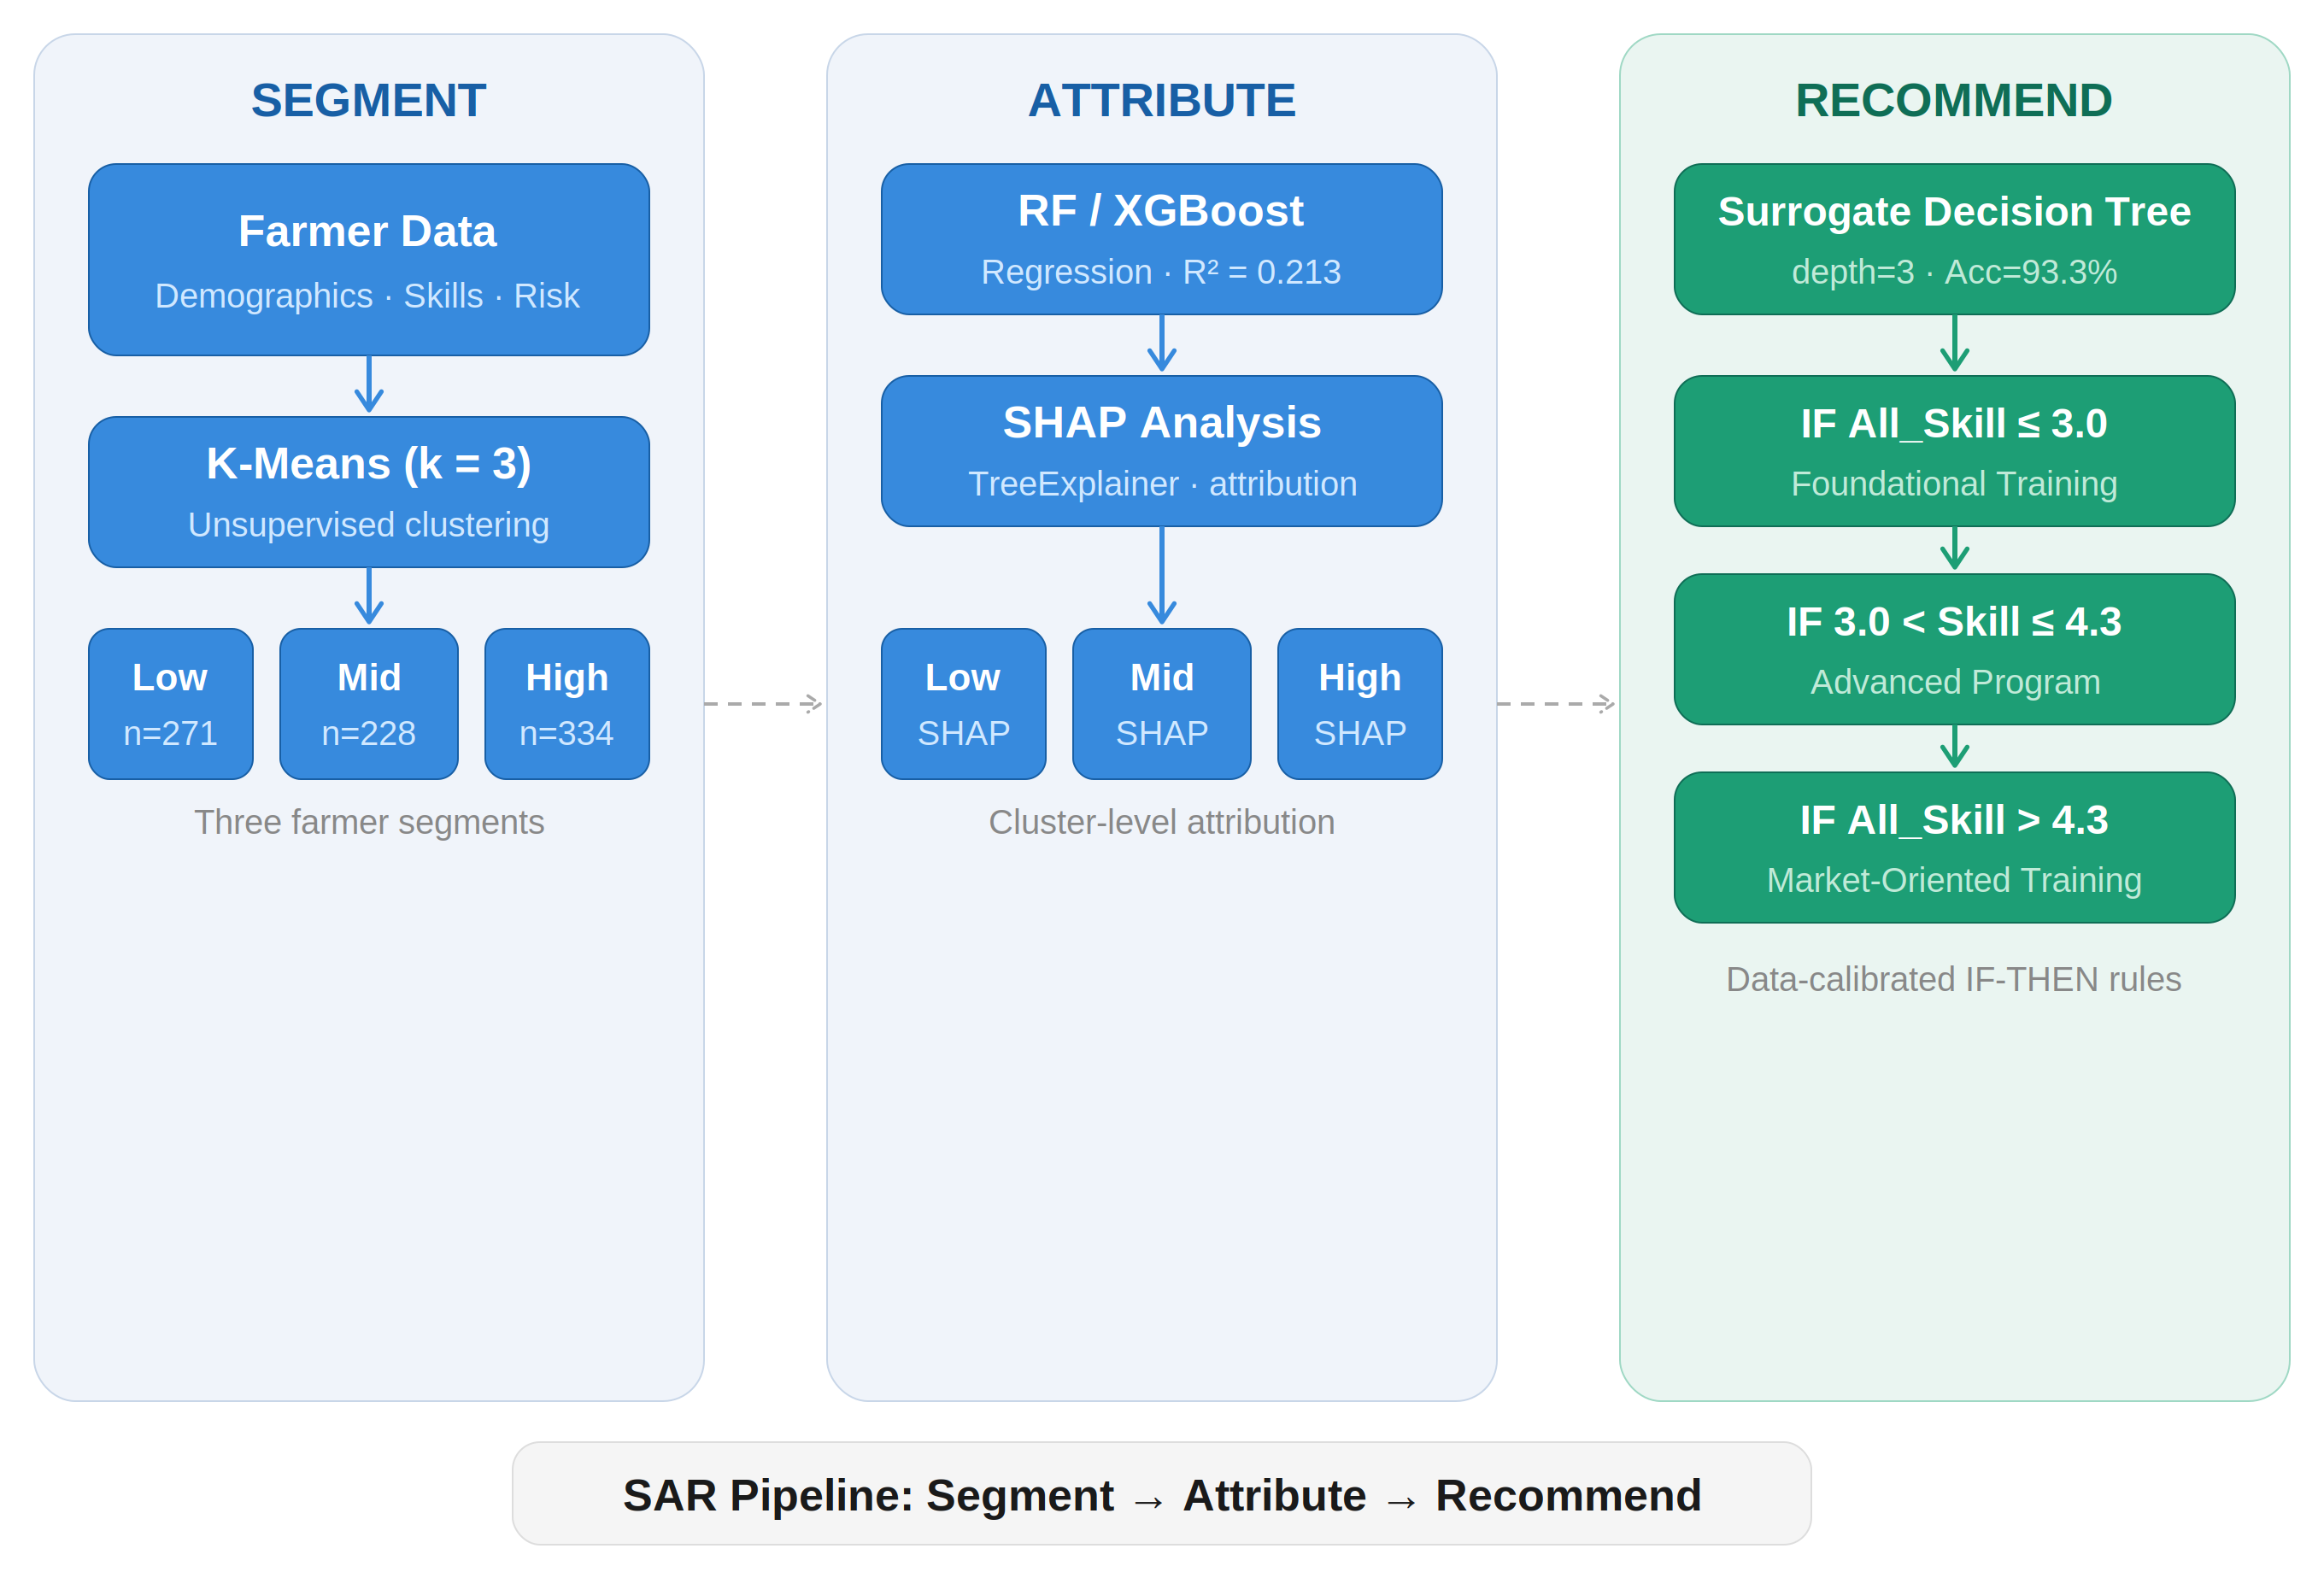
\includegraphics[width=\textwidth]{figures/fig1_framework.png}
\caption{The SAR decision support framework integrating K-Means
segmentation, Random Forest modelling, and SHAP-based explanation
into a unified pipeline for precision agricultural skill development.}
\label{fig:framework}
\end{figure*}

\begin{figure}[htbp]
\centering

\includegraphics[width=\columnwidth]{figures/fig_elbow_silhouette.png}
\caption{Cluster validity analysis using four complementary indices
for $k = 2$--$8$: within-cluster inertia (Elbow), Silhouette,
Calinski--Harabasz (CH), and Davies--Bouldin (DB).
At $k = 3$: Silhouette $= 0.185$, CH $= 202.67$, DB $= 1.835$.}
\label{fig:elbow}
\end{figure}

\begin{figure}[htbp]
\centering

\includegraphics[width=\columnwidth]{figures/fig2_clusters_new.png}
\caption{Farmer segmentation via K-Means ($k = 3$), visualised in
PCA space. Three segments reflect systematic differences in baseline
capabilities and resource access.}
\label{fig:clusters}
\end{figure}

\begin{figure}[htbp]
\centering
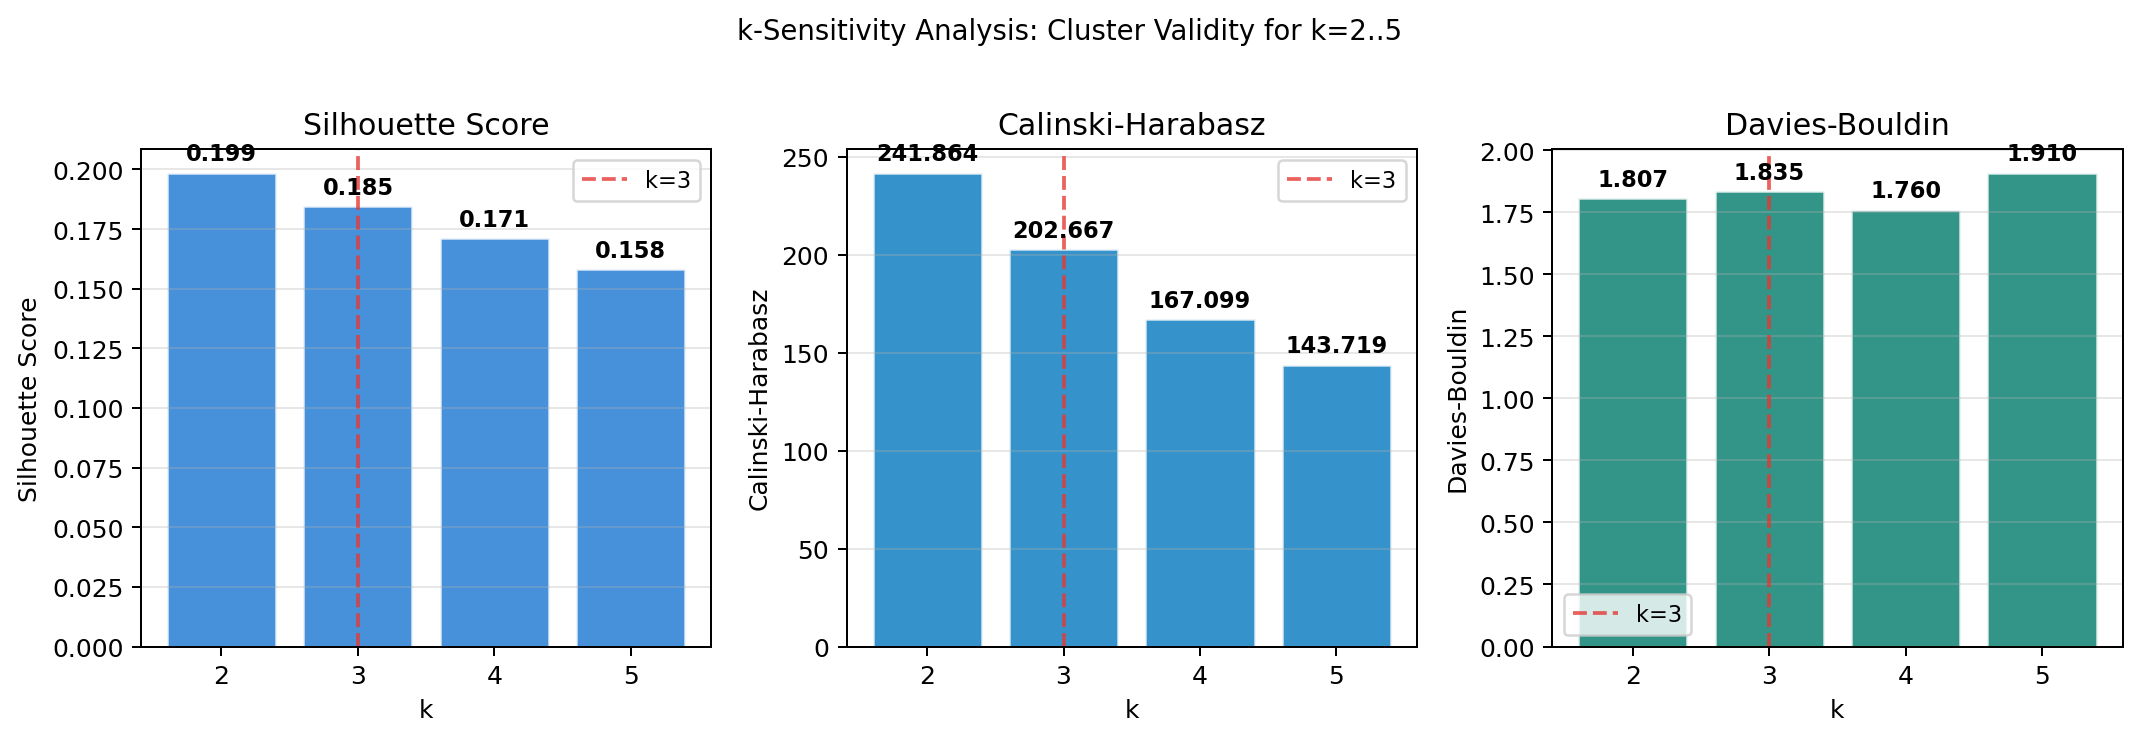
\includegraphics[width=\columnwidth]{figures/fig_k_sensitivity.png}
\caption{K-sensitivity analysis: cluster validity indices (Silhouette,
Calinski--Harabasz, Davies--Bouldin) for $k = 2$--$5$. The dominant
features and qualitative segment distinctions remain stable across all
values of $k$, supporting the robustness of the three-segment solution.}
\label{fig:sensitivity}
\end{figure}

\begin{figure}[htbp]
\centering
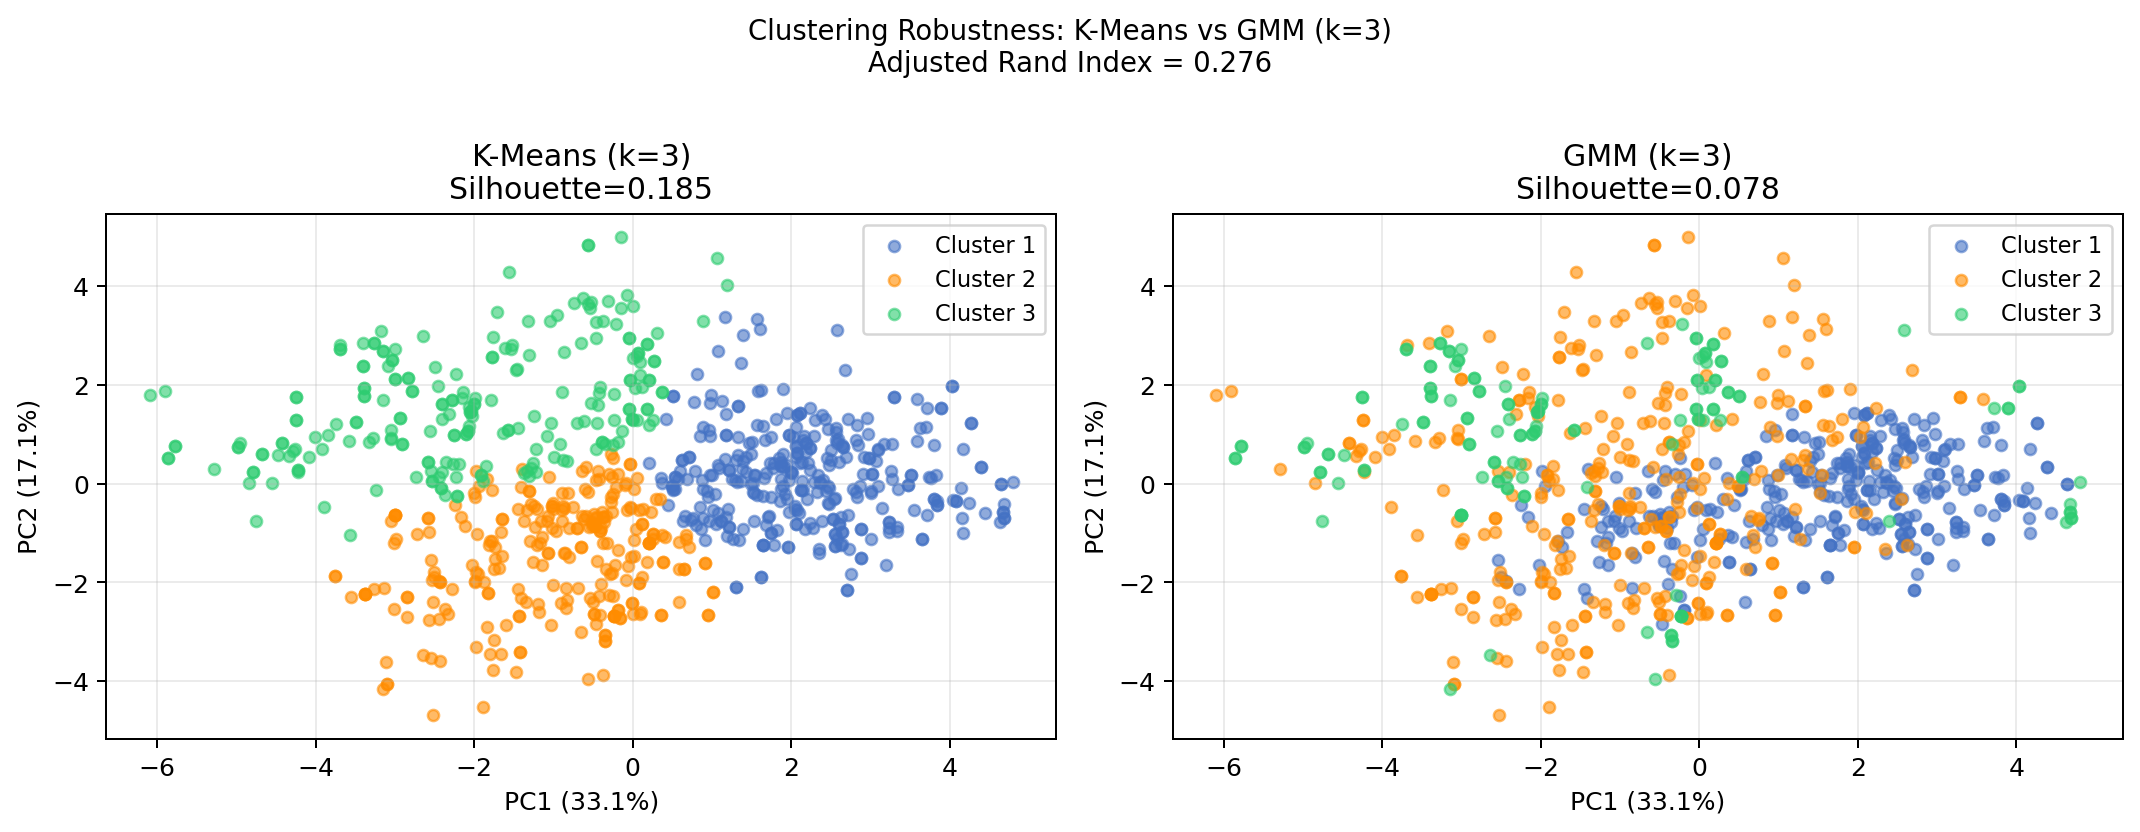
\includegraphics[width=\columnwidth]{figures/fig_gmm_robustness.png}
\caption{Clustering robustness: K-Means versus Gaussian Mixture Model
(GMM) with $k = 3$, visualised in PCA space.
Adjusted Rand Index (ARI) $= 0.28$.
K-Means produces more balanced and interpretable segment groupings
than GMM in this Likert-scale dataset.}
\label{fig:gmm}
\end{figure}

\begin{figure}[htbp]
\centering

\includegraphics[width=\columnwidth]{figures/fig3_importance_new.png}
\caption{Global SHAP-based feature importance (mean $|\text{SHAP}|$)
across all observations ($n = 833$).
\texttt{All\_Skill} is the dominant predictor.}
\label{fig:importance}
\end{figure}

\begin{figure}[htbp]
\centering
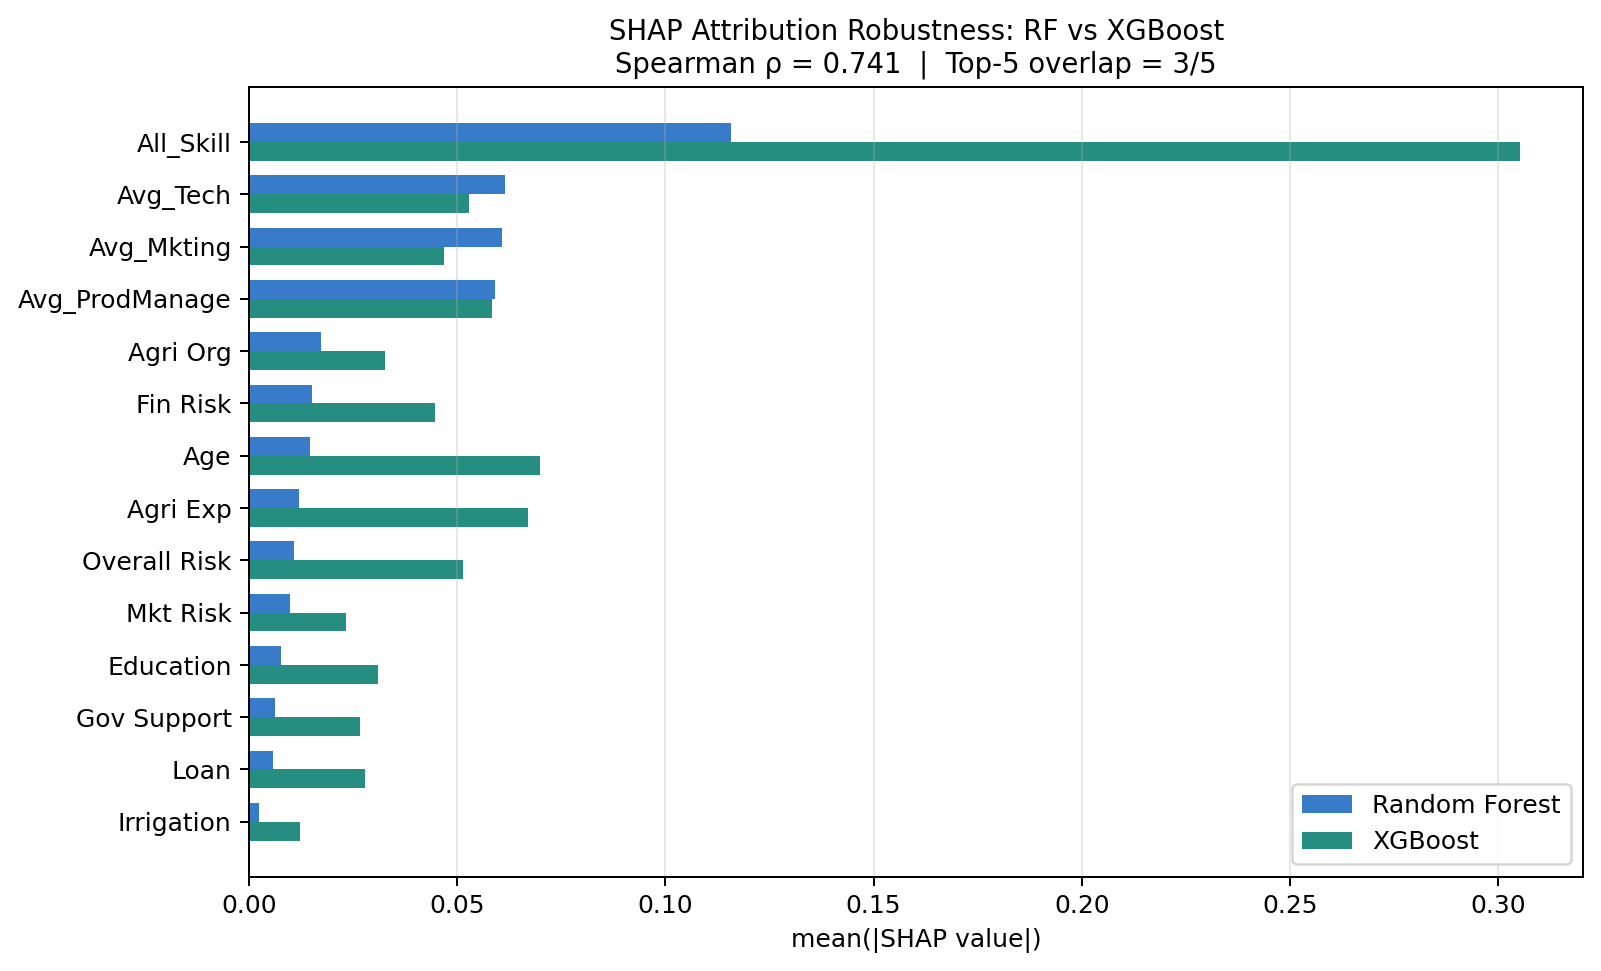
\includegraphics[width=\columnwidth]{figures/fig_shap_robustness.png}
\caption{SHAP attribution robustness: Random Forest versus XGBoost
importance rankings. Spearman $\rho = 0.793$, $p < 0.001$.}
\label{fig:robustness}
\end{figure}

\begin{figure}[htbp]
\centering
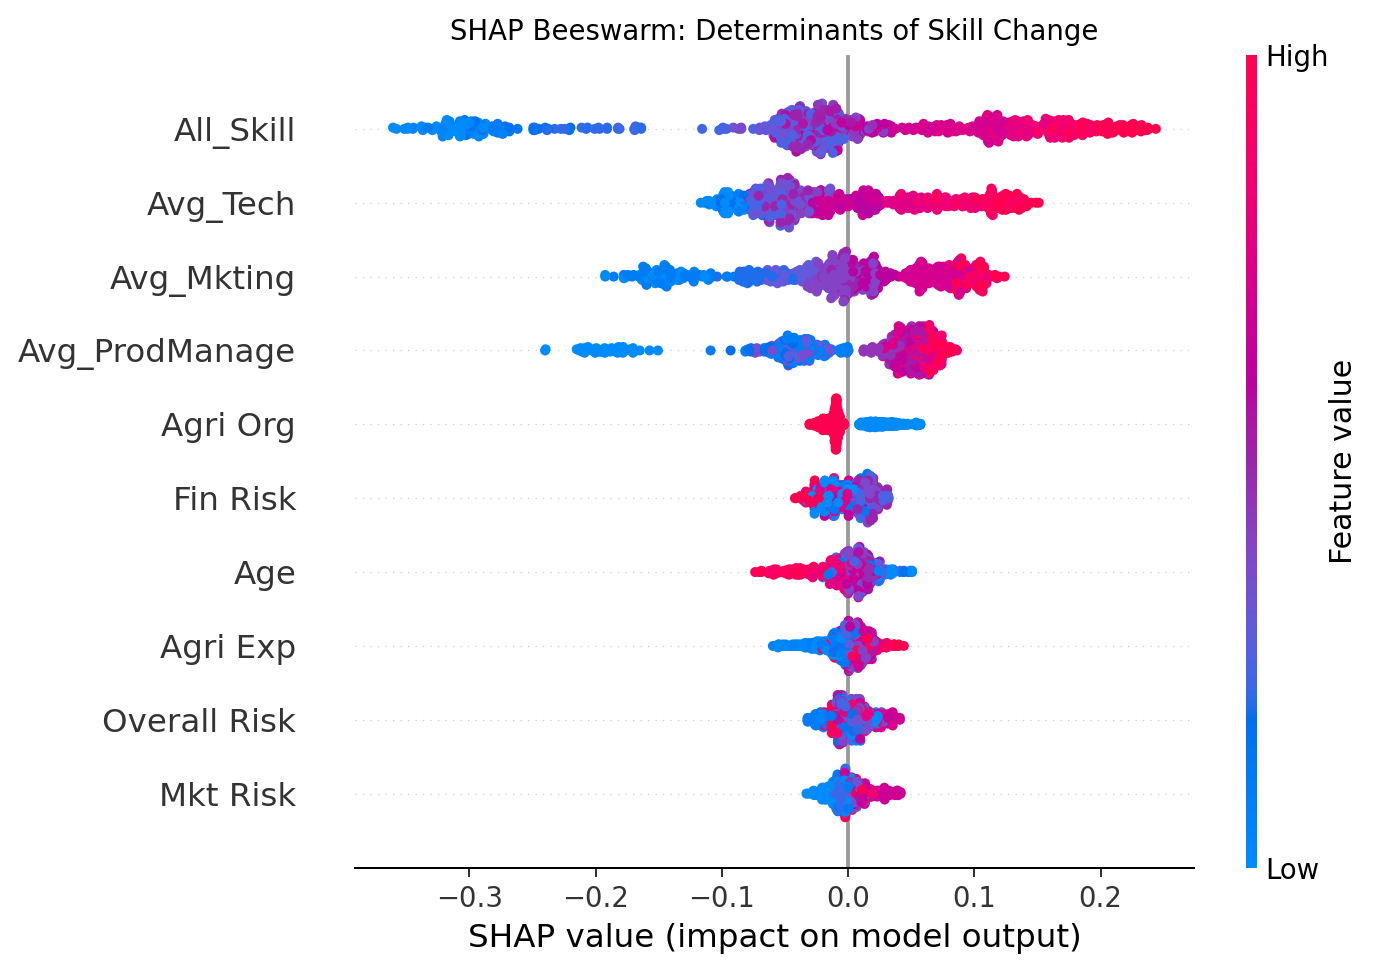
\includegraphics[width=\columnwidth]{figures/fig4_shap_new.png}
\caption{SHAP beeswarm plot showing the distribution and direction
of feature contributions across all observations ($n = 833$).
Colour indicates raw feature value (red $=$ high, blue $=$ low).}
\label{fig:shap}
\end{figure}

\begin{figure*}[htbp]
\centering

\includegraphics[width=\textwidth]{figures/fig4b_cluster_shap_new.png}
\caption{Cluster-stratified SHAP beeswarm plots for the Low-skill
(left, $n = 271$), Moderate-skill (centre, $n = 228$), and High-skill
(right, $n = 334$) segments. Secondary feature importance varies
systematically across segments.}
\label{fig:clusterShap}
\end{figure*}

\begin{figure*}[htbp]
\centering

\includegraphics[width=\textwidth]{figures/fig5_rules_new.png}
\caption{Surrogate decision tree (depth $= 3$, in-sample accuracy
$= 93.3\%$, $n = 817$) fitted on the top-4 SHAP-selected features.
Held-out validation (80/20 split) yields 91.4\% accuracy.
Node labels show the splitting feature, threshold, sample count,
and class distribution.}
\label{fig:rules}
\end{figure*}

%%─────────────────────────────────────────────────────────────────────────────
\section{Discussion}
%%─────────────────────────────────────────────────────────────────────────────

\subsection{Predictive Performance in Context}

The Random Forest achieves $R^{2} = 0.283$ under farmer-level GroupKFold
cross-validation, outperforming both linear and ridge regression baselines
($R^{2} = 0.257$).
This improvement reflects non-linear threshold effects and feature
interactions that additive models cannot capture.
Modest absolute $R^{2}$ values are expected in observational studies of
human learning, where skill change depends heavily on motivation,
engagement, and trainer quality \citep{davis2012}.

Within SAR, the Random Forest serves a structural rather than a purely
predictive role.
\citet{lundberg2020} show that SHAP attributions can remain stable and
informative at moderate predictive accuracy, provided the model captures
meaningful data structure.
This condition is supported here by cross-model attribution agreement
($\rho = 0.793$, Fig.~\ref{fig:robustness}).

Decision logic in SAR is implemented through the surrogate rule structure,
not through point predictions.
The framework's analytical value therefore depends on the consistency of
attribution and rule extraction, not on short-term forecasting precision.

\subsection{Segment-Specific Drivers and Negative Skill Change}

Cluster-level SHAP shows that the determinants of skill change vary
systematically across segments.
This pattern cannot be recovered from global feature importance alone.
Baseline skill (\texttt{All\_Skill}) is the dominant contributor in all
segments, consistent with human capital theory \citep{feder1985,davis2012}.

The negative mean skill change in the Low-skill ($-0.233$) and
Moderate-skill ($-0.105$) segments has two likely causes.
First, regression-to-the-mean: farmers with the lowest initial scores are
more susceptible to downward variation in repeated assessments
\citep{davis2012}.
Second, the voluntary structure of the program leads to lower
participation among Low-skill farmers (28.8\%) compared with High-skill
farmers (69.8\%).
Observed trajectories in lower-skill segments therefore partly reflect
farmers with limited or no training exposure \citep{anderson2004}.

In the High-skill segment, marketing skill (\texttt{Avg\_Mkting}) becomes
more important relative to other predictors.
This suggests that market-oriented competencies are the binding constraint
at higher skill levels, pointing toward advanced market-integration
training for this group.

\subsection{Decision Rule Validity and Generalisation}

The surrogate tree achieves 93.3\% in-sample accuracy.
Farmer-level held-out validation (80/20 split, Option~B) yields 91.4\%
on unseen farmers, and 5-fold GroupKFold CV yields 95.3\% $\pm$ 2.5\%.
The consistent performance across all three approaches confirms that the
decision rules generalise beyond the training data.

The two-stage extraction process---SHAP for feature selection, surrogate
tree for threshold calibration---ensures rules are both theoretically
grounded and empirically calibrated \citep{molnar2022}.
Key thresholds correspond closely to proficiency distinctions within
Thailand's Smart Farmer program, supporting the institutional plausibility
of the results.

Following \citet{rudin2019}, the surrogate rules should be interpreted as
structured decision aids rather than exact reconstructions of the Random
Forest process.

\subsection{Operational Deployment Scenario}

SAR can be implemented as a lightweight, rule-based decision tool.
A typical workflow involves four steps:
\begin{enumerate}
  \item Recording a farmer's baseline profile (demographics, skills, resources)
  \item Assigning the farmer to a segment via K-Means
  \item Applying segment-specific surrogate rules
  \item Generating a structured training recommendation
\end{enumerate}
This process does not require direct model interaction and can be
implemented through a rule-based interface.
The explicit rule structure supports transparency and auditability, which
are key requirements in public-sector extension systems.

Three structural insights emerge from the analysis:
\begin{enumerate}
  \item Pre-training capability is the dominant driver of learning outcomes
  across all segments.
  \item Binding constraints differ by segment: production and education
  limitations dominate at lower skill levels, while marketing competencies
  matter more for advanced farmers.
  \item Uniform training structures are poorly matched to heterogeneous
  populations, as shown by negative or negligible skill change in the Low-
  and Moderate-skill segments.
\end{enumerate}

\subsection{Limitations}

All findings are associative.
Causal interpretation requires randomised or quasi-experimental designs.
The segmentation structure and thresholds are calibrated to the Thai Smart
Farmer population and need recalibration for other contexts.
Low Silhouette scores indicate soft cluster boundaries; segments should
be interpreted as practical groupings rather than sharply separated types.
Held-out validation confirms generalisation, but further prospective field
validation is needed before operational deployment.
Following \citet{rudin2019}, the surrogate model approximates the Random
Forest and should not be treated as an exact replica.

%%─────────────────────────────────────────────────────────────────────────────
\section{Conclusion}
%%─────────────────────────────────────────────────────────────────────────────

This study presents an explainable AI-based decision support system for
precision allocation of agricultural skill development programs, using data
from $n = 833$ farmers in Thailand's Smart Farmer program.

By integrating K-Means segmentation, Random Forest modelling, and SHAP
explainability within the SAR architecture, the framework provides a
deployable and auditable pathway from farmer-level data to structured
training recommendations.
Baseline skill level, production management competency, and educational
attainment are the primary contributors to training outcomes, with their
relative importance varying across segments.
Cluster-level SHAP analysis, validated through cross-model agreement with
XGBoost ($\rho = 0.793$), shows that global feature importance alone is
insufficient for precision training design.

The main methodological contribution is the integration of
cluster-conditioned explainability with surrogate decision tree extraction.
This translates complex model structure into transparent IF--THEN rules
that are interpretable and aligned with observed data patterns.
The surrogate rules generalise well beyond training data, as confirmed
by held-out accuracy (91.4\%) and 5-fold cross-validated accuracy
(95.3\% $\pm$ 2.5\%).

Rather than focusing on predictive accuracy alone, SAR prioritises
structural consistency, interpretability, and operational feasibility.
It offers a practical foundation for modernising agricultural extension
systems through explainable AI.

Future work should focus on (i) expanded out-of-sample validation of
surrogate rules, (ii) quasi-experimental assessment of training effects,
and (iii) integration with real-time agricultural data systems.
Progress on these fronts will strengthen the inferential credibility
and practical scalability of AI-supported agricultural extension
\citep{yang2025,zhang2026}.

%%─────────────────────────────────────────────────────────────────────────────
\section*{Acknowledgements}

The authors thank the Department of Agricultural Extension, Ministry of
Agriculture and Cooperatives, Thailand, for providing access to the Smart
Farmer program dataset under the approved data-sharing agreement.

%%─────────────────────────────────────────────────────────────────────────────
\section*{Data Availability}

The anonymised dataset and analysis code are available from the corresponding
author upon reasonable request, subject to the data-sharing agreement with
the Department of Agricultural Extension, Thailand.

%%─────────────────────────────────────────────────────────────────────────────
\begin{thebibliography}{35}
\expandafter\ifx\csname natexlab\endcsname\relax
  \def\natexlab#1{#1}\fi
\providecommand{\url}[1]{\texttt{#1}}
\providecommand{\href}[2]{#2}
\providecommand{\path}[1]{#1}
\providecommand{\doi}[1]{\href{https://doi.org/#1}{#1}}

\bibitem[{MacQueen(1967)}]{macqueen1967}
MacQueen, J., 1967.
Some methods for classification and analysis of multivariate observations.
In: Proc.\ 5th Berkeley Symposium on Mathematical Statistics and Probability,
vol.\ 1, pp.\ 281--297.

\bibitem[{Feder et~al.(1985)}]{feder1985}
Feder, G., Just, R.E., Zilberman, D., 1985.
Adoption of agricultural innovations in developing countries: A survey.
Economic Development and Cultural Change 33, 255--298.

\bibitem[{Rousseeuw(1987)}]{rouseeuw1987}
Rousseeuw, P.J., 1987.
Silhouettes: A graphical aid to the interpretation and validation of
cluster analysis.
Journal of Computational and Applied Mathematics 20, 53--65.

\bibitem[{Breiman(2001)}]{breiman2001}
Breiman, L., 2001.
Random forests.
Machine Learning 45, 5--32.

\bibitem[{Anderson and Feder(2004)}]{anderson2004}
Anderson, J.R., Feder, G., 2004.
Agricultural extension: Good intentions and hard realities.
World Bank Research Observer 19, 41--60.

\bibitem[{Davis and Franzel(2012)}]{davis2012}
Davis, K., Franzel, S., 2012.
Principles for designing and implementing agricultural extension programs.
Journal of Agricultural Education and Extension 18, 249--263.

\bibitem[{Chen and Guestrin(2016)}]{chen2016}
Chen, T., Guestrin, C., 2016.
XGBoost: A scalable tree boosting system.
In: Proc.\ 22nd ACM SIGKDD, pp.\ 785--794.

\bibitem[{Lundberg and Lee(2017)}]{lundberg2017}
Lundberg, S.M., Lee, S.I., 2017.
A unified approach to interpreting model predictions.
Advances in Neural Information Processing Systems (NeurIPS).

\bibitem[{Ghosal et~al.(2018)}]{ghosal2018}
Ghosal, S., Blystone, D., Singh, A.K., Ganapathysubramanian, B.,
  Singh, A., Sarkar, S., 2018.
An explainable deep machine vision framework for plant stress phenotyping.
PNAS 115, 4613--4618.

\bibitem[{Kamilaris and Prenafeta-Boldu(2018)}]{kamilaris2018}
Kamilaris, A., Prenafeta-Boldu, F.X., 2018.
Deep learning in agriculture: A survey.
Computers and Electronics in Agriculture 147, 70--90.

\bibitem[{Liakos et~al.(2018)}]{liakos2018}
Liakos, K.G., Busato, P., Moshou, D., Pearson, S., Bochtis, D., 2018.
Machine learning in agriculture: A review.
Sensors 18, 2674.

\bibitem[{Guidotti et~al.(2019)}]{guidotti2019}
Guidotti, R., Monreale, A., Ruggieri, S., Turini, F., Giannotti, F.,
  Pedreschi, D., 2019.
A survey of methods for explaining black box models.
ACM Computing Surveys 51(5), 93.

\bibitem[{Rudin(2019)}]{rudin2019}
Rudin, C., 2019.
Stop explaining black box machine learning models for high stakes
decisions and use interpretable models instead.
Nature Machine Intelligence 1, 206--215.

\bibitem[{Arrieta et~al.(2020)}]{arrieta2020}
Arrieta, A.B., Diaz-Rodriguez, N., Del Ser, J., et~al., 2020.
Explainable artificial intelligence (XAI): Concepts, taxonomies,
opportunities and challenges.
Information Fusion 58, 82--115.

\bibitem[{Lundberg et~al.(2020)}]{lundberg2020}
Lundberg, S.M., Erion, G., Chen, H., DeGrave, A., Prutkin, J.M.,
  Nair, B., Katz, R., Himmelfarb, J., Bansal, N., Lee, S.I., 2020.
From local explanations to global understanding with explainable AI
for trees.
Nature Machine Intelligence 2, 56--67.

\bibitem[{Linardatos et~al.(2021)}]{linardatos2021}
Linardatos, P., Papastefanopoulos, V., Kotsiantis, S., 2021.
Explainable AI: A review of machine learning interpretability methods.
Entropy 23(1), 18.

\bibitem[{Ryo(2022)}]{ryo2022}
Ryo, M., 2022.
Explainable artificial intelligence and interpretable machine learning
for agricultural data analysis.
Artificial Intelligence in Agriculture 6, 257--265.

\bibitem[{Hossain et~al.(2022)}]{hossain2022cattle}
Hossain, M.E., Kabir, M.A., Zheng, L., Swain, D.L., McGrath, S.,
  Medway, J., 2022.
A systematic review of machine learning techniques for cattle
identification.
Computers and Electronics in Agriculture 198, 107090.

\bibitem[{Molnar(2022)}]{molnar2022}
Molnar, C., 2022.
Interpretable Machine Learning: A Guide for Making Black-Box Models
Explainable.
\url{https://christophm.github.io/interpretable-ml-book/}

\bibitem[{Ennaji et~al.(2023)}]{ennaji2023nutrient}
Ennaji, O., Vergütz, L., El Allali, A., 2023.
Machine learning in nutrient management: A review.
Computers and Electronics in Agriculture 205, 107623.

\bibitem[{Ghazal et~al.(2024)}]{ghazal2024survey}
Ghazal, S., Munir, A., Qureshi, W.S., 2024.
Computer vision in smart agriculture and precision farming.
Computers and Electronics in Agriculture 214, 108486.

\bibitem[{Omaye et~al.(2024)}]{omaye2024disease}
Omaye, J.D., Ogbuju, E., Ataguba, G., Jaiyeoba, O., Aneke, J.,
  Oladipo, F., 2024.
Cross-comparative review of machine learning for plant disease detection.
Computers and Electronics in Agriculture 212, 108345.

\bibitem[{Wonggasem et~al.(2024)}]{wonggasem2024}
Wonggasem, K., Chakranon, P., Wongchaisuwat, P., 2024.
Automated quality inspection of baby corn using image processing
and deep learning.
Artificial Intelligence in Agriculture 11, 61--69.

\bibitem[{Li et~al.(2025)}]{li2025llm}
Li, H., Wu, H., Li, Q., Zhao, C., 2025.
A review on enhancing agricultural intelligence with large language
models.
Artificial Intelligence in Agriculture 17, 100--125.

\bibitem[{Yang et~al.(2025)}]{yang2025}
Yang, H., et~al., 2025.
AI-driven aquaculture: A review of technological innovations and
sustainable impacts.
Artificial Intelligence in Agriculture 15, 508--525.

\bibitem[{Zhang et~al.(2026)}]{zhang2026}
Zhang, T., et~al., 2026.
Empowering Chinese medicinal agriculture through AI-driven technologies:
A comprehensive review.
Artificial Intelligence in Agriculture. \textit{In press.}

\end{thebibliography}

\end{document}
\documentclass[3p,twocolumn,authoryear]{elsarticle}

\usepackage{natbib}
\usepackage{algorithm}
\usepackage{algpseudocode}
\usepackage{booktabs}
\usepackage{graphicx}
\usepackage{amsmath}
\usepackage{lineno}

\journal{Artificial Intelligence in Agriculture}
\bibliographystyle{elsarticle-harv}

\begin{document}
\begin{frontmatter}

\title{An Explainable AI-based Decision Support System for Precision
       Allocation of Agricultural Skill Development Programs}

\author[inst1]{Kitti Chiewchan\corref{cor1}}
\ead{kitti.ch@bsru.ac.th}
\author[inst2]{Jumtip Seneerattanaprayul}

\cortext[cor1]{Corresponding author}
\address[inst1]{Computer Education, Faculty of Education,
  Bansomdejchaopraya Rajabhat University,
  1061 Issaraphap Road, Hirunrujee, Thonburi, Bangkok 10600, Thailand}
\address[inst2]{Department of Agricultural Economics,
  Faculty of Economics, Kasetsart University,
  50 Ngam Wong Wan Road, Ladyao, Jatujak, Bangkok 10110, Thailand}

\begin{abstract}
The precision allocation of agricultural skill development programs remains
challenging due to heterogeneity among farmer populations and the limitations of
uniform training designs.
This study proposes SAR (Segment--Attribute--Recommend), a transferable
explainable AI architecture that converts SHAP-based attribution into deployable
decision rules for precision training allocation.

The framework combines K-Means clustering for farmer segmentation, Random Forest
regression for modelling skill outcomes, and SHapley Additive exPlanations (SHAP)
for interpretable feature attribution within a three-stage pipeline.
It is applied to panel survey data from $n = 833$ participants in Thailand's Smart
Farmer program.
Three farmer segments are identified---Low-skill, Moderate-skill, and
High-skill---with overall skill level, production management competency, and
educational attainment emerging as the primary determinants of training
effectiveness.

Cluster-level SHAP analysis shows that the importance of these predictors varies
systematically across segments, indicating that global feature importance alone is
insufficient for precision training design \citep{lundberg2020}.
A surrogate decision tree converts SHAP attributions into transparent IF--THEN
rules, allowing extension practitioners to apply data-driven recommendations
without direct interaction with the machine learning model.

Farmer-level held-out validation (80/20 split) yields a classification accuracy of
91.4\%, and 5-fold cross-validated accuracy is 95.3\% $\pm$ 2.5\%.
In-sample surrogate fidelity is 93.3\%.
Prospective validation is recommended before operational deployment.

The SAR architecture offers a deployable and auditable framework for AI-driven
human capital development in agricultural extension systems, subject to
population-specific recalibration.
\end{abstract}

\begin{keyword}
Explainable AI \sep SHAP \sep Decision Support System \sep
Farmer Segmentation \sep Agricultural Extension \sep Machine Learning
\end{keyword}

\end{frontmatter}

\linenumbers

%%─────────────────────────────────────────────────────────────────────────────
\section{Introduction}
%%─────────────────────────────────────────────────────────────────────────────

Agricultural development increasingly relies on data-driven decision-making
as farming systems face rising complexity, environmental variability, and
heterogeneous farmer capabilities.
Over the past decade, advances in machine learning (ML), computer vision,
and sensing technologies have improved automated crop monitoring, disease
detection, nutrient assessment, and livestock management
\citep{kamilaris2018,liakos2018,ghazal2024survey,yang2025}.
These improvements are especially visible in image-based sensing tasks that
span the crop production cycle \citep{ghazal2024survey}.
Complementary reviews cover cattle identification
\citep{hossain2022cattle}, nutrient management \citep{ennaji2023nutrient},
and plant disease detection \citep{omaye2024disease}.

Despite this progress, agricultural AI remains largely fragmented.
Most systems focus on isolated perception tasks without integrating outputs
into broader decision-making workflows
\citep{ghazal2024survey,omaye2024disease}.
This limits their usefulness in real-world settings, particularly where
decisions depend on a combination of environmental, farmer, and management
factors.

Recent work has also explored large language models (LLMs) for knowledge
integration and question-answering in agriculture \citep{li2025llm}.
However, most LLM-based applications remain conceptual and are not yet
connected to field-level decision-support mechanisms.
Challenges such as limited model generalisability and the absence of
standardised datasets persist across domains
\citep{hossain2022cattle,ennaji2023nutrient}.

Agricultural AI can be grouped into three broad clusters:
(A) text-based systems relying on documents and human intermediaries;
(B) perception-centric models driven by image or sensor data; and
(C) interpretability-focused approaches that challenge black-box dominance
in high-stakes decisions.
A common gap across all three is weak integration between perception layers
and actionable decision logic.
The present study addresses this gap in a specific and underserved context.

A particularly underexplored area is AI-driven \textit{human capital
development} in agricultural extension---the allocation of training programs
to heterogeneous farmer populations.
Farmers differ widely in baseline skills, resource access, risk perception,
and learning readiness.
Yet most national extension systems continue to apply standardised curricula
across all participants \citep{anderson2004,feder1985}.
This mismatch leads to uneven outcomes and inefficient use of extension
resources.
Predictive models alone are not sufficient here; extension systems also
require transparent and auditable decision logic that practitioners can use
without specialist AI knowledge \citep{arrieta2020,lundberg2020}.

Explainable AI, and SHapley Additive exPlanations (SHAP) in particular,
offers a principled approach to this problem
\citep{lundberg2017,guidotti2019}.
However, most XAI applications in agriculture stop at post-hoc
interpretation and do not convert explanations into operational rules
\citep{ryo2022,linardatos2021}.
They also rarely address how explainability should vary across farmer
segments, despite evidence that training effectiveness differs
systematically by skill level \citep{davis2012,arrieta2020}.

This study proposes \textbf{SAR (Segment--Attribute--Recommend)}, an
explainable AI architecture for precision allocation of agricultural skill
development programs.
SAR's novelty lies not in its individual components---K-Means, Random
Forest, and SHAP are established methods---but in their integration into
a unified pipeline that operationalises explainability for extension
practice.
Specifically, SAR introduces a cluster-conditioned explainability framework
in which SHAP attribution is localised within farmer segments and
translated into segment-specific decision rules.
To the authors' knowledge, this is the first framework to combine
cluster-stratified SHAP analysis with surrogate rule extraction for
precision training allocation in agricultural extension systems.

%%─────────────────────────────────────────────────────────────────────────────
\section{Literature Review}
%%─────────────────────────────────────────────────────────────────────────────

\subsection{Machine Learning and Computer Vision in Agriculture}

ML and computer vision have become central to modern precision agriculture,
supporting crop monitoring, disease detection, yield estimation, and
livestock identification.
\citet{ghazal2024survey} show that image-based sensing remains the dominant
modality across the crop production cycle.
CNN-based architectures generally outperform classical ML for cattle
identification when training data are adequate
\citep{hossain2022cattle}.
Random Forest and deep learning models are widely used for nutrient
prediction \citep{ennaji2023nutrient}.
For plant disease detection, deep learning does not always outperform
classical ML, highlighting the importance of choosing methods based on
data characteristics \citep{omaye2024disease}.
Beyond research settings, ML has also improved operational tasks such as
quality inspection and grading in production systems
\citep{wonggasem2024}.

Taken together, these studies show rapid progress in perception-centric
applications but limited integration with downstream decision processes.
This motivates a need for architectures that extend beyond sensing tasks
and provide interpretable, actionable guidance for practitioners.

\subsection{Explainable AI for Agricultural Decision Support}

As ML models grow more complex, explainable AI (XAI) has become a core
requirement for transparency and accountability in agricultural systems
\citep{arrieta2020,linardatos2021}.
\citet{guidotti2019} provide a taxonomy of explanation methods, covering
feature attribution, surrogate modelling, and rule extraction---all three
of which underpin SAR.

SHAP has become the most widely used technique for explaining tree-based
models due to its grounding in cooperative game theory \citep{lundberg2017}.
\citet{lundberg2020} show that SHAP attributions remain stable across
different tree architectures, including Random Forest and XGBoost.
In agriculture, SHAP has been applied to yield prediction, disease
diagnosis, and risk assessment \citep{ghosal2018,ryo2022}.
Notably, \citet{ryo2022} call for frameworks that translate XAI outputs
into actionable decision structures---a gap addressed by SAR.

However, most XAI studies in agriculture remain descriptive.
They offer post-hoc insights but do not convert explanations into
operational rules \citep{linardatos2021,arrieta2020}.
The integration of XAI with farmer segmentation for segment-specific
attribution remains largely unexplored.

\subsection{Farmer Heterogeneity and Training Effectiveness}

Research consistently shows that farmers differ in baseline skills,
resource endowments, and risk profiles, leading to uneven responses to
extension programs \citep{feder1985,anderson2004}.
Farmers with stronger pre-training competencies tend to benefit more from
advanced training \citep{davis2012}.
Yet most extension systems still use standardised curricula due to
operational constraints and the absence of targeting tools
\citep{anderson2004}.
SAR addresses this directly by providing a data-driven mechanism for
segment-aware allocation.

\subsection{Large Language Models in Agricultural Intelligence}

Recent work highlights the potential of LLMs for integrating fragmented
agricultural knowledge through fine-tuning and knowledge-aware reasoning
\citep{li2025llm}.
However, most current applications remain conceptual.
SAR differs by focusing on empirical, field-level decision mechanisms
grounded in observed training outcomes.

\subsection{Research Gaps}

Five gaps motivate the present study:

\begin{enumerate}
  \item \textbf{From explanation to decision logic.}
  Most XAI applications stop at post-hoc insights without translating them
  into rules for extension practice.

  \item \textbf{Lack of segment-aware decision pipelines.}
  Existing systems rarely integrate segmentation, predictive modelling,
  and interpretable rule extraction into a deployable pipeline.

  \item \textbf{Limited cluster-conditioned explainability.}
  SHAP is typically applied at the global level, ignoring systematic
  differences across farmer segments.

  \item \textbf{Weak integration of attribution with decision layers.}
  Few studies connect attribution mechanisms with rule-based decision
  structures.

  \item \textbf{Human-centred interpretability is underexamined.}
  Evidence on how non-technical stakeholders use explanations in practice
  remains limited.
\end{enumerate}

SAR is designed to address gaps~1--3 by localising SHAP attribution within
segments and translating these attributions into surrogate rules for
extension practice.

%%─────────────────────────────────────────────────────────────────────────────
\section{Methodology}
%%─────────────────────────────────────────────────────────────────────────────

\subsection{Data and Study Context}

The dataset consists of panel survey data from farmers in Thailand's Smart
Farmer program, collected between 2018 and 2020.
The program targets smallholder farmers across five regions and assesses
five skill domains: production management, input management, technology
adoption, analysis and planning, and marketing.
Pre- and post-training assessments used validated 5-point Likert-scale
instruments administered by certified extension officers.
The primary outcome, $Ch\_Skill$, is the difference between post-training
and pre-training composite skill scores.

Missing data were limited (all features $<$ 5\%).
Binary and asset-related variables were imputed with zero, reflecting
that asset absence is a valid zero-value observation.
Continuous Likert-scale variables were imputed with column means, which
is appropriate given their approximately symmetric distributions.
All numeric predictors were standardised to zero mean and unit variance.
Sensitivity checks using median imputation produced no substantive
changes in model performance or SHAP rankings.

\textit{Ethics and data access:}
The survey was conducted under institutional research protocols of the
Department of Agricultural Extension, Ministry of Agriculture and
Cooperatives, Thailand.
All records were anonymised prior to analysis under a formal
data-sharing agreement, and no personally identifiable information was
used.
Informed consent was obtained during Smart Farmer program registration.
A data access statement is provided in the supplementary materials.

\subsection{Farmer Segmentation}

K-Means clustering \citep{macqueen1967} was applied to 15 baseline
features capturing skill levels, demographics, and risk perceptions.
The feature set includes \textit{age, education, agricultural experience,
irrigation access, loan access, average production management skill,
average input management skill, average technology adoption skill,
average analysis and planning skill, average marketing skill, average
networking skill, production risk perception, input risk perception,
market risk perception,} and \textit{financial risk perception}.

Cluster validity was assessed using four complementary indices
\citep{rouseeuw1987}: within-cluster inertia (Elbow method), Silhouette,
Calinski--Harabasz (CH), and Davies--Bouldin (DB).
The Elbow curve (Fig.~\ref{fig:elbow}) shows a clear inflection at
$k = 3$. At this value, Silhouette $= 0.185$, CH $= 202.67$, and
DB $= 1.835$.
Although Silhouette is modest, this is expected for Likert-scale survey
data, which rarely satisfies the compactness assumptions of
distance-based metrics \citep{rouseeuw1987}.
All indices show consistently weak separation across $k = 2$--$8$,
suggesting this reflects intrinsic data properties rather than a poor
choice of $k$.
The DB score at $k = 3$ is close to the global minimum at $k = 4$,
supporting a meaningful partition.

To verify the stability of this solution, two robustness checks were
performed.
First, a k-sensitivity analysis evaluated cluster structure for
$k = 2$--$5$ (Fig.~\ref{fig:sensitivity}).
The dominant features and qualitative distinctions among segments remained
consistent across all tested values.
Second, a Gaussian Mixture Model (GMM) with $k = 3$ was estimated as an
alternative (Fig.~\ref{fig:gmm}).
The Adjusted Rand Index (ARI) between K-Means and GMM solutions was 0.28,
indicating partial structural agreement.
GMM produced less balanced segment sizes and showed lower internal
validity (Silhouette $= 0.078$), while K-Means yielded more
interpretable and domain-consistent groupings.
These checks support the use of K-Means with $k = 3$ as a practically
meaningful and stable segmentation approach.

The selection of $k = 3$ is further supported by domain alignment.
Thailand's Smart Farmer program formally recognises three proficiency
tiers (Smart Farmer, Smart Farmer in Progress, and Knowledge Farmer),
making a three-segment structure directly actionable in practice.

\subsection{Predictive Modelling}

A Random Forest regression model \citep{breiman2001} was used to predict
$Ch\_Skill$ using 18 features spanning demographics, baseline skills,
risk perception, and program participation.
To prevent data leakage in the panel dataset---where each farmer
contributes two observations (pre- and post-training)---all
cross-validation was performed using GroupKFold with 5 folds, grouping
by farmer ID.
This ensures that both observations from the same farmer are always
assigned to the same fold.
XGBoost \citep{chen2016} was trained on the same feature set as a
robustness check.

\subsection{Baseline Models and Performance Evaluation}

OLS and ridge regression were estimated as baselines.
Performance was measured using $R^{2}$, RMSE, and MAE under 5-fold
GroupKFold cross-validation.
Random Forest hyperparameters were optimised by grid search over
\texttt{n\_estimators} $\in$ \{300, 500\},
\texttt{max\_depth} $\in$ \{5, 8, None\},
\texttt{min\_samples\_leaf} $\in$ \{5, 10, 20\}, and
\texttt{max\_features} $\in$ \{\texttt{sqrt}, 0.5\}, using the same
5-fold GroupKFold strategy (nested CV is noted as a limitation).
Optimal parameters: \texttt{n\_estimators} $= 500$,
\texttt{min\_samples\_leaf} $= 10$,
\texttt{max\_features} $=$ \texttt{sqrt}.
Table~\ref{tab:baseline_performance} reports results.

\begin{table}[htbp]
\centering
\caption{5-fold GroupKFold cross-validated performance ($n = 833$,
grouped by farmer ID). Values in parentheses are standard deviations
across folds.}
\label{tab:baseline_performance}
\begin{tabular}{@{}lccc@{}}
\toprule
\textbf{Model} & \textbf{$R^{2}$} & \textbf{RMSE} & \textbf{MAE} \\
\midrule
Linear Regression  & 0.257 (0.028) & 0.599 & 0.468 \\
Ridge Regression   & 0.257 (0.028) & 0.599 & 0.468 \\
\textbf{RF (ours)} & \textbf{0.283 (0.036)} & \textbf{0.588} & \textbf{0.455} \\
\bottomrule
\end{tabular}
\end{table}

Within SAR, the Random Forest serves a primarily \textit{structural}
role rather than a purely predictive one.
It provides the basis for SHAP-based attribution analysis rather than
standalone forecasting.
As shown by \citet{lundberg2020}, SHAP attributions can be stable and
informative even when predictive accuracy is modest, provided the model
captures meaningful non-linear relationships.
The observed $R^{2} = 0.283$ indicates that the Random Forest captures
non-linear and interaction effects in skill change that go beyond what
linear models explain.

\subsection{Explainable AI Analysis}

SHAP values were computed using TreeExplainer \citep{lundberg2017} to
quantify each feature's marginal contribution to predicted
$Ch\_Skill$ values.
Global importance was defined as mean absolute SHAP value across all
observations \citep{lundberg2020}.
Cluster-level SHAP analysis was then conducted to identify segment-specific
drivers of skill improvement, corresponding to the \textit{Attribute}
stage of SAR.

Attribution stability was assessed by replicating the SHAP analysis
using XGBoost \citep{chen2016} on the same feature set.
Agreement was measured using Spearman rank correlation.

\subsection{Decision Support Framework}

The SAR pipeline follows three stages (Fig.~\ref{fig:framework}).
In the \textit{Segment} stage, farmers are assigned to one of three
groups via K-Means.
In the \textit{Attribute} stage, cluster-level SHAP values identify the
most important features within each segment.
In the \textit{Recommend} stage, these attributions are converted into
IF--THEN rules using a surrogate decision tree.

\subsection{Rule Extraction Method}

Rule extraction proceeds in two steps.

In Step~1 (feature selection), mean absolute SHAP values within each
cluster identify which features enter the rule conditions.
The top $K = 4$ features were selected, capturing more than 85\% of
total SHAP attribution mass in each cluster.

In Step~2 (threshold calibration), a surrogate decision tree (depth~$= 3$)
is fitted on the SHAP-selected features to derive data-driven thresholds
\citep{guidotti2019,molnar2022}.

The binary target labels farmers in the High-skill cluster as having
\textit{high training potential}, and farmers in the Low- and
Moderate-skill clusters as having \textit{low or moderate training
potential}.
This framing reflects the goal of identifying farmers most likely to
benefit from advanced training.

This is not circular reasoning.
Clustering uses only baseline features describing initial farmer
characteristics.
The supervised model and SHAP analysis operate on observed skill change
($Ch\_Skill$).
The surrogate tree approximates the SHAP-informed decision boundary using
a reduced feature set, not the clustering itself.

Classification accuracy is reported for the full training sample
($n = 817$; 16 observations excluded due to missing values in
SHAP-selected features).
Cross-validated accuracy and held-out validation metrics are also reported
to assess generalisation.
Prospective field validation remains a priority for future work.

To assess whether the surrogate rules generalise beyond the training data,
an 80/20 train--test split was applied at the farmer level (Option~B).
The surrogate tree was trained on the 80\% training subset using cluster
assignments derived from that subset only.
Test farmers were assigned to the nearest centroid from the training
K-Means model.
This ensures that the held-out set contains no information used during
training.

The procedure is summarised in Algorithm~\ref{alg:rules}.

\begin{algorithm}
\caption{SHAP-guided Surrogate Rule Extraction}
\label{alg:rules}
\begin{algorithmic}[1]
\Require Cluster assignments $C$, SHAP matrix $S$, feature matrix $X$,
         tree depth $d = 3$, top-$K = 4$
\Ensure Set of IF--THEN rules $\mathcal{R}$
\State $\mathcal{R} \gets \emptyset$
\For{each cluster $c$ in $C$}
  \State $\phi_j \gets \text{mean}(|S_{c,j}|)$
         \Comment{Mean absolute SHAP per feature}
  \State $\mathcal{F}_c \gets \text{Top-}4(\phi)$
  \State Fit surrogate tree $T_c$ on $X[\mathcal{F}_c]$
  \State Extract rules $\mathcal{R}_c$ from leaf paths of $T_c$
  \State $\mathcal{R} \gets \mathcal{R} \cup \mathcal{R}_c$
\EndFor
\State \Return $\mathcal{R}$
\end{algorithmic}
\end{algorithm}

\subsection{Clustering Robustness}

Alternative values of $k$ from 2 to 8 were evaluated.
The dominant features and qualitative distinctions among the Low-skill,
Moderate-skill, and High-skill groups remained stable across all tested
values.
This supports the robustness of the segmentation within the SAR pipeline.

%%─────────────────────────────────────────────────────────────────────────────
\section{Results}
%%─────────────────────────────────────────────────────────────────────────────

\subsection{Ablation Study}

An ablation study assessed the contribution of each SAR component.
The full framework was compared with two simplified baselines.

The first baseline uses clustering only, applying a threshold on baseline
skill (\texttt{All\_Skill}) to approximate training allocation without
ML attribution.
The second uses Random Forest predictions without segmentation, applying
a global threshold to infer training potential.

As shown in Table~\ref{tab:ablation}, the full SAR framework achieves the
highest accuracy (93.3\%), outperforming both the clustering-only baseline
(89.1\%) and the RF-only approach (79.3\%).

The clustering-only method performs reasonably well because baseline skill
is the dominant predictor.
However, it cannot capture non-linear interactions and does not produce
segment-specific decision rules.
The RF-only model lacks the segmentation structure needed for
policy-oriented support.
These results confirm that effective decision support requires the joint
integration of all three SAR components.

\begin{table}[htbp]
\centering
\caption{Ablation study: SAR versus simplified baselines.}
\label{tab:ablation}
\resizebox{\columnwidth}{!}{
\begin{tabular}{@{}llc@{}}
\toprule
\textbf{Model} & \textbf{Description} & \textbf{Accuracy} \\
\midrule
Clustering-only & Baseline skill threshold & 89.1\% \\
RF (no seg.)    & Global prediction threshold & 79.3\% \\
\textbf{SAR (proposed)} & Segmentation + SHAP + rules & \textbf{93.3\%} \\
\bottomrule
\end{tabular}
}
\end{table}

\subsection{Farmer Segmentation}

K-Means with $k = 3$ identifies three distinct farmer segments, shown in
PCA space in Fig.~\ref{fig:clusters}.
Cluster validity is confirmed by four complementary indices: Silhouette
$= 0.185$, CH $= 202.67$, DB $= 1.835$ (Fig.~\ref{fig:elbow}).
Table~\ref{tab:cluster_profile} summarises the mean profile of each
segment.

Clustering robustness was evaluated using k-sensitivity analysis
(Fig.~\ref{fig:sensitivity}) and GMM comparison
(Fig.~\ref{fig:gmm}).
The three-segment structure remained stable across $k = 2$--$5$, with
the dominant features consistent in each case.
The GMM solution (ARI $= 0.28$ relative to K-Means) produced less
balanced and less interpretable groupings, supporting the preference
for K-Means in this context.

The \textbf{Low-skill} cluster ($n = 271$) comprises older farmers
(mean age 54.9 years) with the lowest educational attainment (mean 2.9)
and weakest baseline skills.
This segment shows a negative mean skill change ($Ch\_Skill = -0.233$),
consistent with regression-to-the-mean effects in repeated assessments
\citep{davis2012}.
This highlights the need for foundational training designs for this group.

The \textbf{Moderate-skill} cluster ($n = 228$) has intermediate
competencies and the highest market risk perception (mean 3.23).
The near-zero skill change ($Ch\_Skill = -0.105$) suggests that standard
training yields limited gains here, pointing to the need for more
differentiated program design \citep{anderson2004}.

The \textbf{High-skill} cluster ($n = 334$) has the strongest baseline
competencies, the highest Smart Farmer participation rate (69.8\%), and
the only positive mean skill change ($Ch\_Skill = +0.259$).
This pattern is consistent with human capital theory
\citep{feder1985,davis2012}.

\begin{table*}[htbp]
\centering
\caption{Cluster profile: mean variable values by farmer segment
($n = 833$). Skill scales: 1--5 Likert. Between-cluster differences
are statistically significant (Kruskal--Wallis, $p < 0.001$).}
\label{tab:cluster_profile}
\begin{tabular}{@{}lcccccccc@{}}
\toprule
\textbf{Segment} & \textbf{n} & \textbf{All\_Skill}
  & \textbf{Ch\_Skill} & \textbf{Age}
  & \textbf{Education} & \textbf{ProdManage}
  & \textbf{Tech} & \textbf{SF Rate} \\
\midrule
Low-skill      & 271 & 3.06 & $-$0.233 & 54.9 & 2.9 & 3.58 & 3.05 & 28.8\% \\
Moderate-skill & 228 & 3.26 & $-$0.105 & 50.6 & 3.8 & 3.42 & 3.22 & 51.3\% \\
High-skill     & 334 & 4.27 & $+$0.259 & 52.6 & 3.7 & 4.46 & 4.40 & 69.8\% \\
\bottomrule
\end{tabular}
\end{table*}

\subsection{Predictive Performance}

The optimised Random Forest achieves $R^{2} = 0.283$ under 5-fold
GroupKFold cross-validation (Table~\ref{tab:baseline_performance}),
outperforming both linear and ridge regression baselines
($R^{2} = 0.257$).
The modest absolute values reflect the influence of unobserved factors
such as motivation and trainer quality on human learning outcomes
\citep{davis2012}.
XGBoost yields comparable performance ($R^{2} \approx 0.27$),
supporting robustness of the predictive component \citep{chen2016}.

\subsection{Global SHAP Importance and Attribution Robustness}

Global SHAP-based feature importance is shown in Fig.~\ref{fig:importance}.
Overall baseline skill (\texttt{All\_Skill}) is the dominant predictor,
followed by production management skill (\texttt{Avg\_ProdManage}),
education (\texttt{edu}), marketing skill (\texttt{Avg\_Mkting}), and
irrigation access (\texttt{irriga}).

The prominence of \texttt{All\_Skill} aligns with human capital theory
\citep{feder1985}.
Secondary contributions suggest that technical skill and education
moderate training uptake.
Training-type variables contribute relatively little, indicating that
what farmers bring to training matters more than the training modality
itself \citep{ryo2022}.

Attribution robustness was assessed by replicating the SHAP analysis
using XGBoost.
As shown in Fig.~\ref{fig:robustness}, the Spearman rank correlation
between global importance vectors is $\rho = 0.793$ ($p < 0.001$), with
three features appearing in both top-four rankings.
This confirms that the reported attributions reflect data structure rather
than model-specific artefacts \citep{lundberg2020}.

\subsection{SHAP Beeswarm Analysis}

The SHAP beeswarm plot (Fig.~\ref{fig:shap}) shows feature contribution
patterns across observations.
For \texttt{All\_Skill}, higher values produce positive contributions and
lower values produce negative contributions, forming a near-monotonic
relationship.
For \texttt{irriga}, predominantly negative contributions suggest that
farmers with irrigation access may already have stronger baselines,
resulting in smaller measured gains.
These patterns confirm that the model captures non-linear relationships
that linear coefficients cannot represent.

\subsection{Cluster-Level SHAP Analysis}

Cluster-stratified SHAP plots are shown in Fig.~\ref{fig:clusterShap}.
\texttt{All\_Skill} remains the dominant predictor across all segments,
but secondary drivers vary systematically.

In the \textbf{Low-skill} cluster, low production management skill and
education produce strongly negative contributions.
In the \textbf{Moderate-skill} cluster, contributions are more evenly
spread across features.
In the \textbf{High-skill} cluster, marketing skill (\texttt{Avg\_Mkting})
becomes relatively more important.

Attribution stability is higher for the Low- and Moderate-skill segments
than for the High-skill segment, indicating greater uncertainty in
secondary drivers for advanced farmers.
These results confirm that global feature importance alone is insufficient
for precision training allocation.

\subsection{Decision Rule Extraction and Validation}

A surrogate decision tree (depth $= 3$) was fitted on the top-4
SHAP-selected features (Fig.~\ref{fig:rules}).
In-sample classification accuracy is 93.3\% ($n = 817$).

To assess generalisation, a farmer-level 80/20 train--test split
(Option~B) was applied.
The surrogate tree was trained on 80\% of farmers (n $= 320$) using
cluster assignments derived from that subset only.
Test farmers (n $= 81$) were assigned to the nearest K-Means centroid.
The held-out accuracy was \textbf{91.4\%}, with precision and recall
balanced across both classes (F1 $\approx 0.91$ for both Low/Moderate
and High groups).

Five-fold GroupKFold cross-validation on the full dataset yielded an
average accuracy of \textbf{95.3\% $\pm$ 2.5\%}.

These results are summarised in Table~\ref{tab:surr_validation}.
The consistent performance across all three evaluation approaches
confirms that the extracted rules generalise beyond the training data
and are not artefacts of in-sample overfitting.

\begin{table}[htbp]
\centering
\caption{Surrogate decision tree validation results.}
\label{tab:surr_validation}
\begin{tabular}{@{}lcc@{}}
\toprule
\textbf{Evaluation method} & \textbf{n} & \textbf{Accuracy} \\
\midrule
In-sample (full dataset)        & 817 & 93.3\% \\
Train set (80\% farmers)        & 320 & 95.9\% \\
Held-out test (20\% farmers)    &  81 & \textbf{91.4\%} \\
5-fold GroupKFold CV            & 817 & 95.3\% $\pm$ 2.5\% \\
\bottomrule
\end{tabular}
\end{table}

These data-calibrated thresholds provide transparent and auditable
decision rules suitable for use by extension practitioners.

%%─── Figures ────────────────────────────────────────────────────────────────

\begin{figure*}[htbp]
\centering
\includegraphics[width=\textwidth]{figures/fig1_framework_new.png}
\caption{The SAR decision support framework integrating K-Means
segmentation, Random Forest modelling, and SHAP-based explanation
into a unified pipeline for precision agricultural skill development.}
\label{fig:framework}
\end{figure*}

\begin{figure}[htbp]
\centering

\includegraphics[width=\columnwidth]{figures/fig_elbow_silhouette.png}
\caption{Cluster validity analysis using four complementary indices
for $k = 2$--$8$: within-cluster inertia (Elbow), Silhouette,
Calinski--Harabasz (CH), and Davies--Bouldin (DB).
At $k = 3$: Silhouette $= 0.185$, CH $= 202.67$, DB $= 1.835$.}
\label{fig:elbow}
\end{figure}

\begin{figure}[htbp]
\centering

\includegraphics[width=\columnwidth]{figures/fig2_clusters_new.png}
\caption{Farmer segmentation via K-Means ($k = 3$), visualised in
PCA space. Three segments reflect systematic differences in baseline
capabilities and resource access.}
\label{fig:clusters}
\end{figure}

\begin{figure}[htbp]
\centering
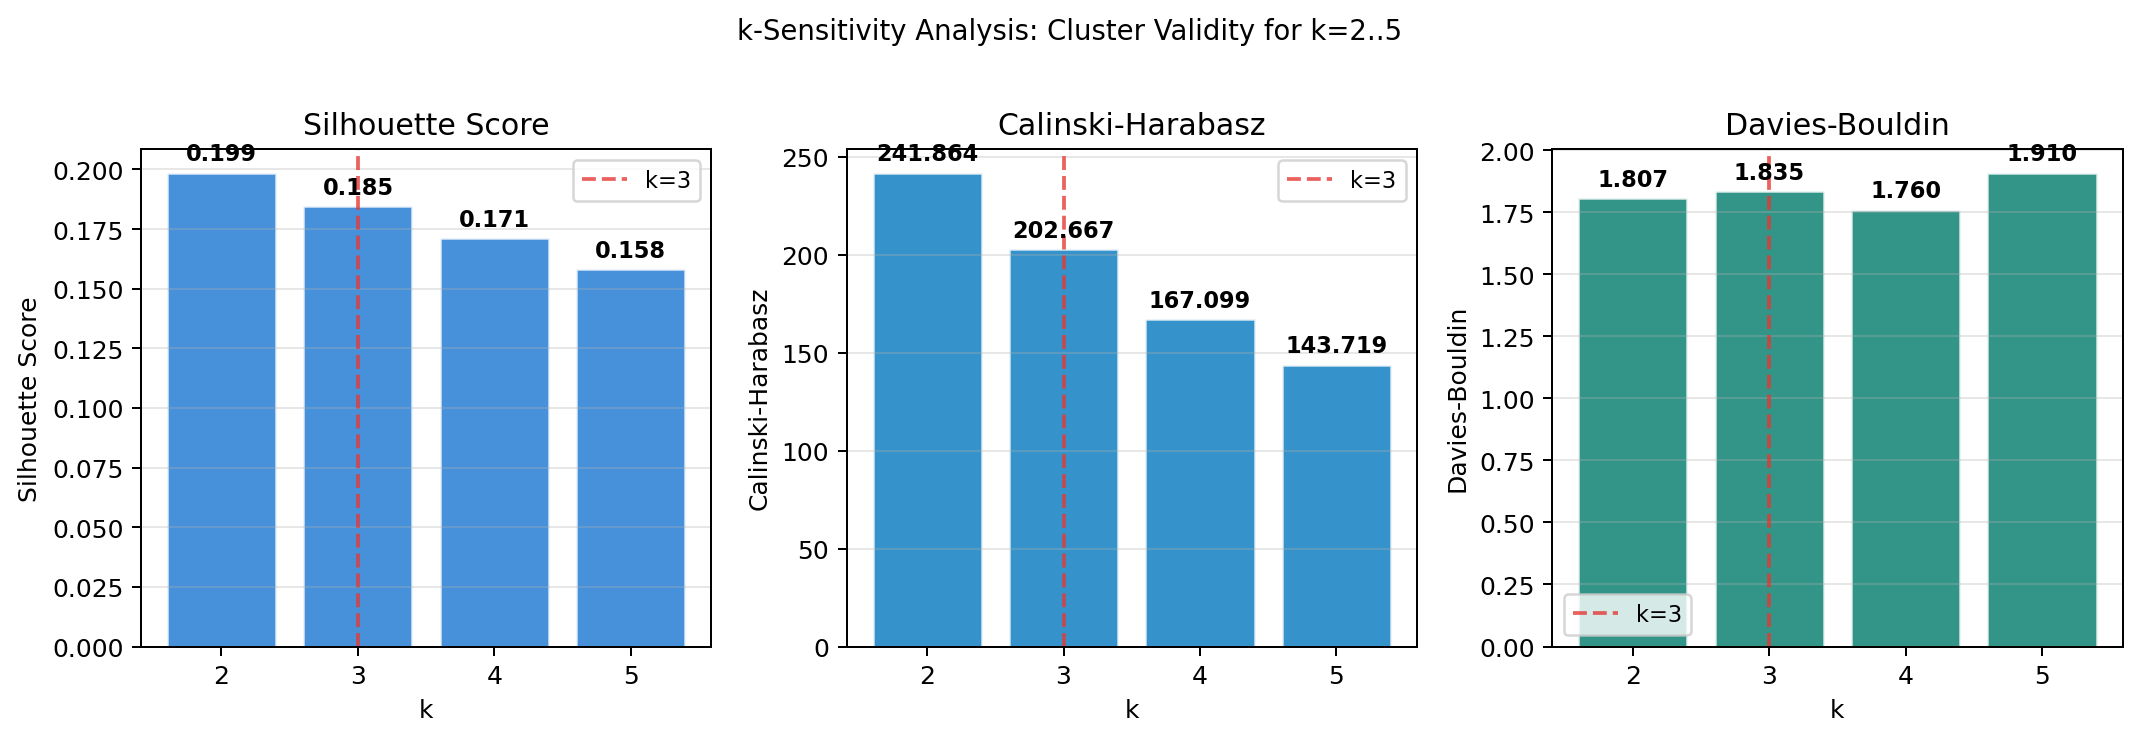
\includegraphics[width=\columnwidth]{figures/fig_k_sensitivity.png}
\caption{K-sensitivity analysis: cluster validity indices (Silhouette,
Calinski--Harabasz, Davies--Bouldin) for $k = 2$--$5$. The dominant
features and qualitative segment distinctions remain stable across all
values of $k$, supporting the robustness of the three-segment solution.}
\label{fig:sensitivity}
\end{figure}

\begin{figure}[htbp]
\centering
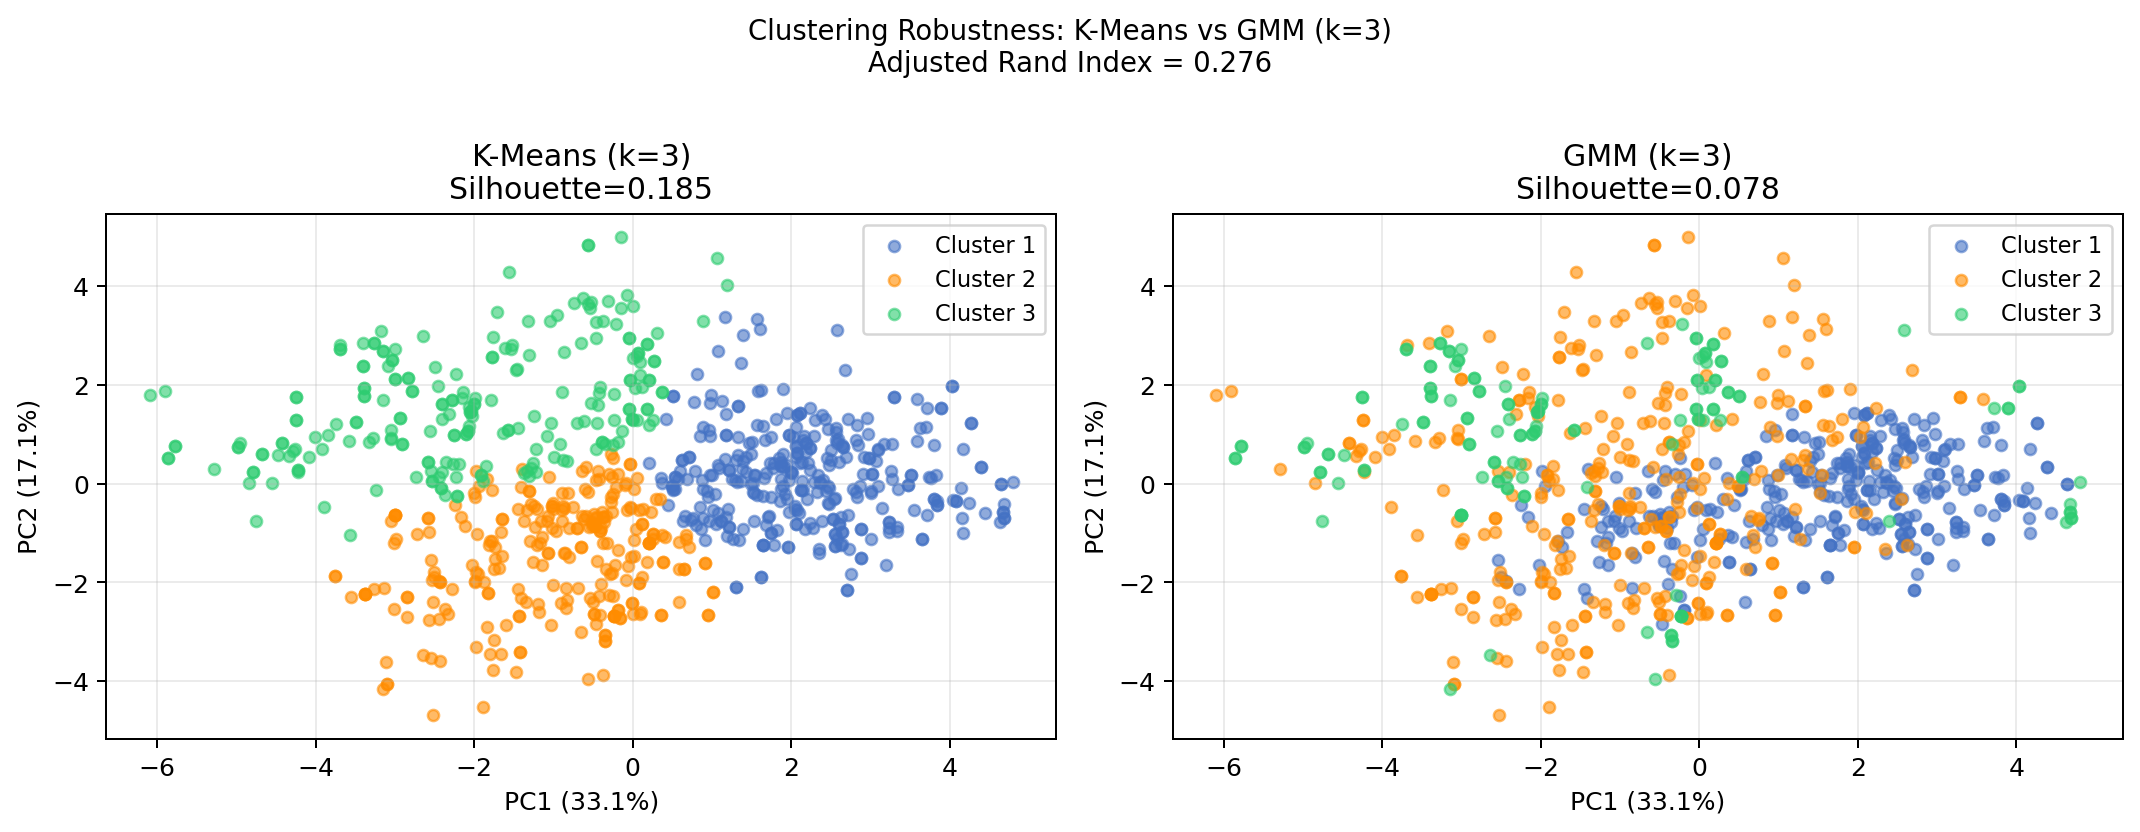
\includegraphics[width=\columnwidth]{figures/fig_gmm_robustness.png}
\caption{Clustering robustness: K-Means versus Gaussian Mixture Model
(GMM) with $k = 3$, visualised in PCA space.
Adjusted Rand Index (ARI) $= 0.28$.
K-Means produces more balanced and interpretable segment groupings
than GMM in this Likert-scale dataset.}
\label{fig:gmm}
\end{figure}

\begin{figure}[htbp]
\centering

\includegraphics[width=\columnwidth]{figures/fig3_importance_new.png}
\caption{Global SHAP-based feature importance (mean $|\text{SHAP}|$)
across all observations ($n = 833$).
\texttt{All\_Skill} is the dominant predictor.}
\label{fig:importance}
\end{figure}

\begin{figure}[htbp]
\centering
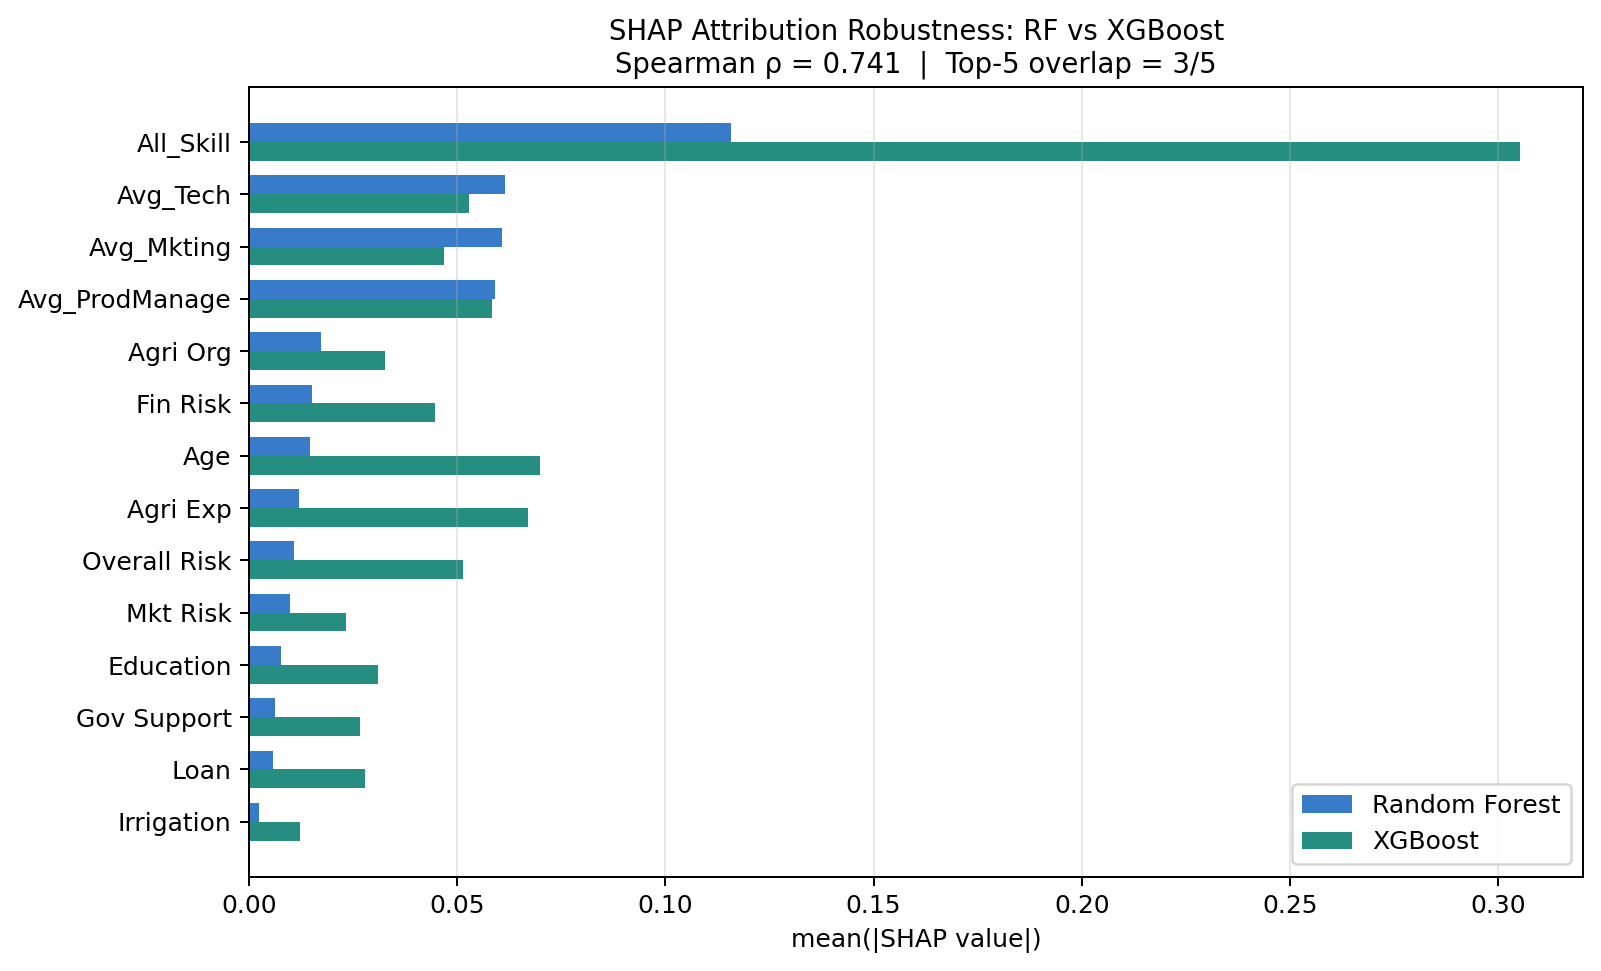
\includegraphics[width=\columnwidth]{figures/fig_shap_robustness.png}
\caption{SHAP attribution robustness: Random Forest versus XGBoost
importance rankings. Spearman $\rho = 0.793$, $p < 0.001$.}
\label{fig:robustness}
\end{figure}

\begin{figure}[htbp]
\centering
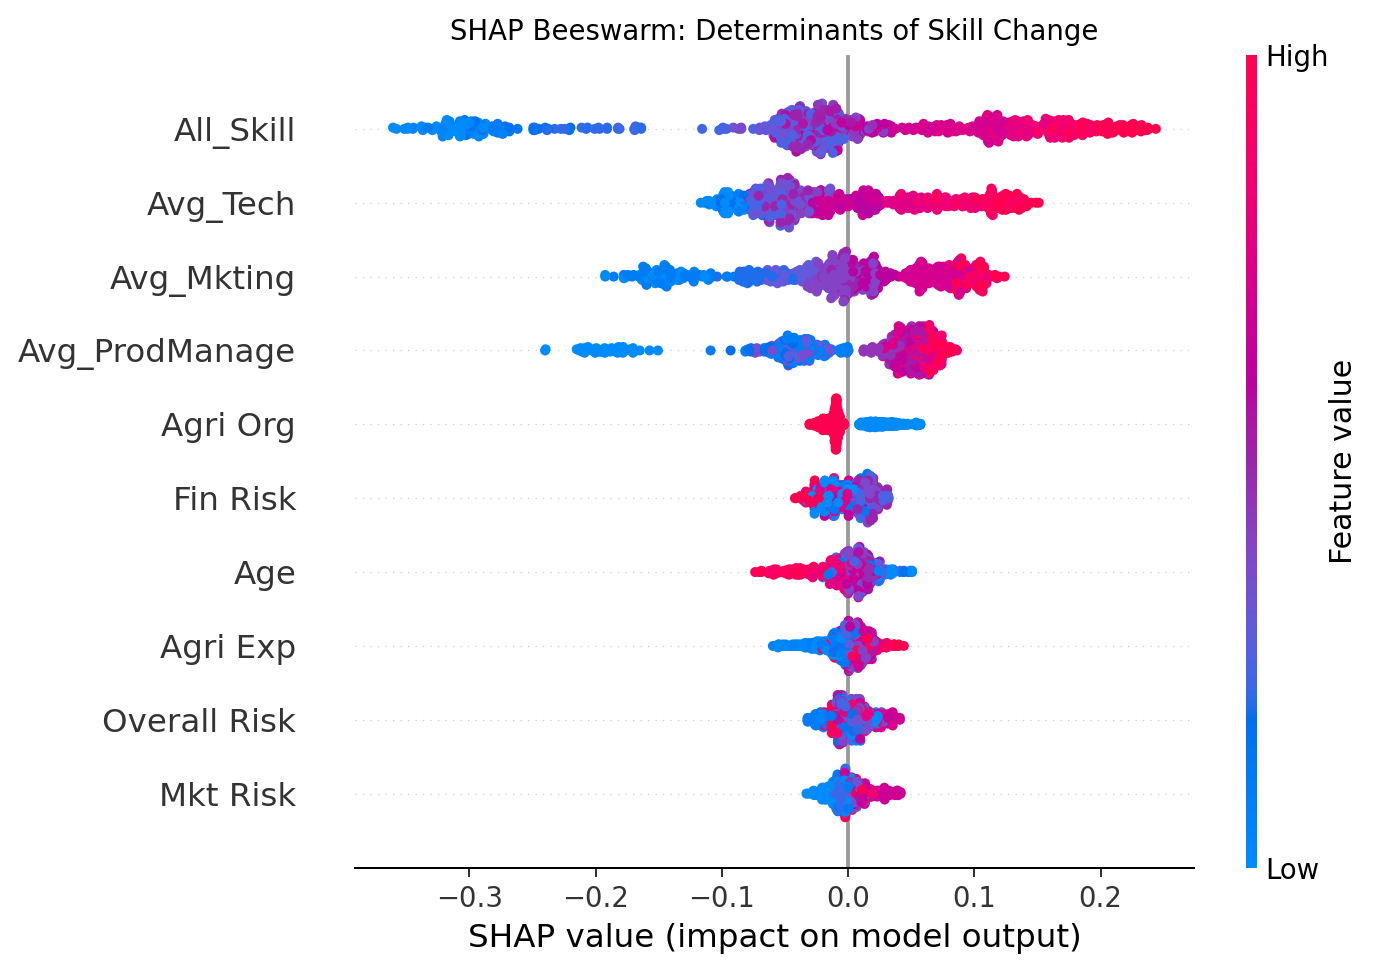
\includegraphics[width=\columnwidth]{figures/fig4_shap_new.png}
\caption{SHAP beeswarm plot showing the distribution and direction
of feature contributions across all observations ($n = 833$).
Colour indicates raw feature value (red $=$ high, blue $=$ low).}
\label{fig:shap}
\end{figure}

\begin{figure*}[htbp]
\centering

\includegraphics[width=\textwidth]{figures/fig4b_cluster_shap_new.png}
\caption{Cluster-stratified SHAP beeswarm plots for the Low-skill
(left, $n = 271$), Moderate-skill (centre, $n = 228$), and High-skill
(right, $n = 334$) segments. Secondary feature importance varies
systematically across segments.}
\label{fig:clusterShap}
\end{figure*}

\begin{figure*}[htbp]
\centering

\includegraphics[width=\textwidth]{figures/fig5_rules_new.png}
\caption{Surrogate decision tree (depth $= 3$, in-sample accuracy
$= 93.3\%$, $n = 817$) fitted on the top-4 SHAP-selected features.
Held-out validation (80/20 split) yields 91.4\% accuracy.
Node labels show the splitting feature, threshold, sample count,
and class distribution.}
\label{fig:rules}
\end{figure*}

%%─────────────────────────────────────────────────────────────────────────────
\section{Discussion}
%%─────────────────────────────────────────────────────────────────────────────

\subsection{Predictive Performance in Context}

The Random Forest achieves $R^{2} = 0.283$ under farmer-level GroupKFold
cross-validation, outperforming both linear and ridge regression baselines
($R^{2} = 0.257$).
This improvement reflects non-linear threshold effects and feature
interactions that additive models cannot capture.
Modest absolute $R^{2}$ values are expected in observational studies of
human learning, where skill change depends heavily on motivation,
engagement, and trainer quality \citep{davis2012}.

Within SAR, the Random Forest serves a structural rather than a purely
predictive role.
\citet{lundberg2020} show that SHAP attributions can remain stable and
informative at moderate predictive accuracy, provided the model captures
meaningful data structure.
This condition is supported here by cross-model attribution agreement
($\rho = 0.793$, Fig.~\ref{fig:robustness}).

Decision logic in SAR is implemented through the surrogate rule structure,
not through point predictions.
The framework's analytical value therefore depends on the consistency of
attribution and rule extraction, not on short-term forecasting precision.

\subsection{Segment-Specific Drivers and Negative Skill Change}

Cluster-level SHAP shows that the determinants of skill change vary
systematically across segments.
This pattern cannot be recovered from global feature importance alone.
Baseline skill (\texttt{All\_Skill}) is the dominant contributor in all
segments, consistent with human capital theory \citep{feder1985,davis2012}.

The negative mean skill change in the Low-skill ($-0.233$) and
Moderate-skill ($-0.105$) segments has two likely causes.
First, regression-to-the-mean: farmers with the lowest initial scores are
more susceptible to downward variation in repeated assessments
\citep{davis2012}.
Second, the voluntary structure of the program leads to lower
participation among Low-skill farmers (28.8\%) compared with High-skill
farmers (69.8\%).
Observed trajectories in lower-skill segments therefore partly reflect
farmers with limited or no training exposure \citep{anderson2004}.

In the High-skill segment, marketing skill (\texttt{Avg\_Mkting}) becomes
more important relative to other predictors.
This suggests that market-oriented competencies are the binding constraint
at higher skill levels, pointing toward advanced market-integration
training for this group.

\subsection{Decision Rule Validity and Generalisation}

The surrogate tree achieves 93.3\% in-sample accuracy.
Farmer-level held-out validation (80/20 split, Option~B) yields 91.4\%
on unseen farmers, and 5-fold GroupKFold CV yields 95.3\% $\pm$ 2.5\%.
The consistent performance across all three approaches confirms that the
decision rules generalise beyond the training data.

The two-stage extraction process---SHAP for feature selection, surrogate
tree for threshold calibration---ensures rules are both theoretically
grounded and empirically calibrated \citep{molnar2022}.
Key thresholds correspond closely to proficiency distinctions within
Thailand's Smart Farmer program, supporting the institutional plausibility
of the results.

Following \citet{rudin2019}, the surrogate rules should be interpreted as
structured decision aids rather than exact reconstructions of the Random
Forest process.

\subsection{Operational Deployment Scenario}

SAR can be implemented as a lightweight, rule-based decision tool.
A typical workflow involves four steps:
\begin{enumerate}
  \item Recording a farmer's baseline profile (demographics, skills, resources)
  \item Assigning the farmer to a segment via K-Means
  \item Applying segment-specific surrogate rules
  \item Generating a structured training recommendation
\end{enumerate}
This process does not require direct model interaction and can be
implemented through a rule-based interface.
The explicit rule structure supports transparency and auditability, which
are key requirements in public-sector extension systems.

Three structural insights emerge from the analysis:
\begin{enumerate}
  \item Pre-training capability is the dominant driver of learning outcomes
  across all segments.
  \item Binding constraints differ by segment: production and education
  limitations dominate at lower skill levels, while marketing competencies
  matter more for advanced farmers.
  \item Uniform training structures are poorly matched to heterogeneous
  populations, as shown by negative or negligible skill change in the Low-
  and Moderate-skill segments.
\end{enumerate}

\subsection{Limitations}

All findings are associative.
Causal interpretation requires randomised or quasi-experimental designs.
The segmentation structure and thresholds are calibrated to the Thai Smart
Farmer population and need recalibration for other contexts.
Low Silhouette scores indicate soft cluster boundaries; segments should
be interpreted as practical groupings rather than sharply separated types.
Held-out validation confirms generalisation, but further prospective field
validation is needed before operational deployment.
Following \citet{rudin2019}, the surrogate model approximates the Random
Forest and should not be treated as an exact replica.

%%─────────────────────────────────────────────────────────────────────────────
\section{Conclusion}
%%─────────────────────────────────────────────────────────────────────────────

This study presents an explainable AI-based decision support system for
precision allocation of agricultural skill development programs, using data
from $n = 833$ farmers in Thailand's Smart Farmer program.

By integrating K-Means segmentation, Random Forest modelling, and SHAP
explainability within the SAR architecture, the framework provides a
deployable and auditable pathway from farmer-level data to structured
training recommendations.
Baseline skill level, production management competency, and educational
attainment are the primary contributors to training outcomes, with their
relative importance varying across segments.
Cluster-level SHAP analysis, validated through cross-model agreement with
XGBoost ($\rho = 0.793$), shows that global feature importance alone is
insufficient for precision training design.

The main methodological contribution is the integration of
cluster-conditioned explainability with surrogate decision tree extraction.
This translates complex model structure into transparent IF--THEN rules
that are interpretable and aligned with observed data patterns.
The surrogate rules generalise well beyond training data, as confirmed
by held-out accuracy (91.4\%) and 5-fold cross-validated accuracy
(95.3\% $\pm$ 2.5\%).

Rather than focusing on predictive accuracy alone, SAR prioritises
structural consistency, interpretability, and operational feasibility.
It offers a practical foundation for modernising agricultural extension
systems through explainable AI.

Future work should focus on (i) expanded out-of-sample validation of
surrogate rules, (ii) quasi-experimental assessment of training effects,
and (iii) integration with real-time agricultural data systems.
Progress on these fronts will strengthen the inferential credibility
and practical scalability of AI-supported agricultural extension
\citep{yang2025,zhang2026}.

%%─────────────────────────────────────────────────────────────────────────────
\section*{Acknowledgements}

The authors thank the Department of Agricultural Extension, Ministry of
Agriculture and Cooperatives, Thailand, for providing access to the Smart
Farmer program dataset under the approved data-sharing agreement.

%%─────────────────────────────────────────────────────────────────────────────
\section*{Data Availability}

The anonymised dataset and analysis code are available from the corresponding
author upon reasonable request, subject to the data-sharing agreement with
the Department of Agricultural Extension, Thailand.

%%─────────────────────────────────────────────────────────────────────────────
\begin{thebibliography}{35}
\expandafter\ifx\csname natexlab\endcsname\relax
  \def\natexlab#1{#1}\fi
\providecommand{\url}[1]{\texttt{#1}}
\providecommand{\href}[2]{#2}
\providecommand{\path}[1]{#1}
\providecommand{\doi}[1]{\href{https://doi.org/#1}{#1}}

\bibitem[{MacQueen(1967)}]{macqueen1967}
MacQueen, J., 1967.
Some methods for classification and analysis of multivariate observations.
In: Proc.\ 5th Berkeley Symposium on Mathematical Statistics and Probability,
vol.\ 1, pp.\ 281--297.

\bibitem[{Feder et~al.(1985)}]{feder1985}
Feder, G., Just, R.E., Zilberman, D., 1985.
Adoption of agricultural innovations in developing countries: A survey.
Economic Development and Cultural Change 33, 255--298.

\bibitem[{Rousseeuw(1987)}]{rouseeuw1987}
Rousseeuw, P.J., 1987.
Silhouettes: A graphical aid to the interpretation and validation of
cluster analysis.
Journal of Computational and Applied Mathematics 20, 53--65.

\bibitem[{Breiman(2001)}]{breiman2001}
Breiman, L., 2001.
Random forests.
Machine Learning 45, 5--32.

\bibitem[{Anderson and Feder(2004)}]{anderson2004}
Anderson, J.R., Feder, G., 2004.
Agricultural extension: Good intentions and hard realities.
World Bank Research Observer 19, 41--60.

\bibitem[{Davis and Franzel(2012)}]{davis2012}
Davis, K., Franzel, S., 2012.
Principles for designing and implementing agricultural extension programs.
Journal of Agricultural Education and Extension 18, 249--263.

\bibitem[{Chen and Guestrin(2016)}]{chen2016}
Chen, T., Guestrin, C., 2016.
XGBoost: A scalable tree boosting system.
In: Proc.\ 22nd ACM SIGKDD, pp.\ 785--794.

\bibitem[{Lundberg and Lee(2017)}]{lundberg2017}
Lundberg, S.M., Lee, S.I., 2017.
A unified approach to interpreting model predictions.
Advances in Neural Information Processing Systems (NeurIPS).

\bibitem[{Ghosal et~al.(2018)}]{ghosal2018}
Ghosal, S., Blystone, D., Singh, A.K., Ganapathysubramanian, B.,
  Singh, A., Sarkar, S., 2018.
An explainable deep machine vision framework for plant stress phenotyping.
PNAS 115, 4613--4618.

\bibitem[{Kamilaris and Prenafeta-Boldu(2018)}]{kamilaris2018}
Kamilaris, A., Prenafeta-Boldu, F.X., 2018.
Deep learning in agriculture: A survey.
Computers and Electronics in Agriculture 147, 70--90.

\bibitem[{Liakos et~al.(2018)}]{liakos2018}
Liakos, K.G., Busato, P., Moshou, D., Pearson, S., Bochtis, D., 2018.
Machine learning in agriculture: A review.
Sensors 18, 2674.

\bibitem[{Guidotti et~al.(2019)}]{guidotti2019}
Guidotti, R., Monreale, A., Ruggieri, S., Turini, F., Giannotti, F.,
  Pedreschi, D., 2019.
A survey of methods for explaining black box models.
ACM Computing Surveys 51(5), 93.

\bibitem[{Rudin(2019)}]{rudin2019}
Rudin, C., 2019.
Stop explaining black box machine learning models for high stakes
decisions and use interpretable models instead.
Nature Machine Intelligence 1, 206--215.

\bibitem[{Arrieta et~al.(2020)}]{arrieta2020}
Arrieta, A.B., Diaz-Rodriguez, N., Del Ser, J., et~al., 2020.
Explainable artificial intelligence (XAI): Concepts, taxonomies,
opportunities and challenges.
Information Fusion 58, 82--115.

\bibitem[{Lundberg et~al.(2020)}]{lundberg2020}
Lundberg, S.M., Erion, G., Chen, H., DeGrave, A., Prutkin, J.M.,
  Nair, B., Katz, R., Himmelfarb, J., Bansal, N., Lee, S.I., 2020.
From local explanations to global understanding with explainable AI
for trees.
Nature Machine Intelligence 2, 56--67.

\bibitem[{Linardatos et~al.(2021)}]{linardatos2021}
Linardatos, P., Papastefanopoulos, V., Kotsiantis, S., 2021.
Explainable AI: A review of machine learning interpretability methods.
Entropy 23(1), 18.

\bibitem[{Ryo(2022)}]{ryo2022}
Ryo, M., 2022.
Explainable artificial intelligence and interpretable machine learning
for agricultural data analysis.
Artificial Intelligence in Agriculture 6, 257--265.

\bibitem[{Hossain et~al.(2022)}]{hossain2022cattle}
Hossain, M.E., Kabir, M.A., Zheng, L., Swain, D.L., McGrath, S.,
  Medway, J., 2022.
A systematic review of machine learning techniques for cattle
identification.
Computers and Electronics in Agriculture 198, 107090.

\bibitem[{Molnar(2022)}]{molnar2022}
Molnar, C., 2022.
Interpretable Machine Learning: A Guide for Making Black-Box Models
Explainable.
\url{https://christophm.github.io/interpretable-ml-book/}

\bibitem[{Ennaji et~al.(2023)}]{ennaji2023nutrient}
Ennaji, O., Vergütz, L., El Allali, A., 2023.
Machine learning in nutrient management: A review.
Computers and Electronics in Agriculture 205, 107623.

\bibitem[{Ghazal et~al.(2024)}]{ghazal2024survey}
Ghazal, S., Munir, A., Qureshi, W.S., 2024.
Computer vision in smart agriculture and precision farming.
Computers and Electronics in Agriculture 214, 108486.

\bibitem[{Omaye et~al.(2024)}]{omaye2024disease}
Omaye, J.D., Ogbuju, E., Ataguba, G., Jaiyeoba, O., Aneke, J.,
  Oladipo, F., 2024.
Cross-comparative review of machine learning for plant disease detection.
Computers and Electronics in Agriculture 212, 108345.

\bibitem[{Wonggasem et~al.(2024)}]{wonggasem2024}
Wonggasem, K., Chakranon, P., Wongchaisuwat, P., 2024.
Automated quality inspection of baby corn using image processing
and deep learning.
Artificial Intelligence in Agriculture 11, 61--69.

\bibitem[{Li et~al.(2025)}]{li2025llm}
Li, H., Wu, H., Li, Q., Zhao, C., 2025.
A review on enhancing agricultural intelligence with large language
models.
Artificial Intelligence in Agriculture 17, 100--125.

\bibitem[{Yang et~al.(2025)}]{yang2025}
Yang, H., et~al., 2025.
AI-driven aquaculture: A review of technological innovations and
sustainable impacts.
Artificial Intelligence in Agriculture 15, 508--525.

\bibitem[{Zhang et~al.(2026)}]{zhang2026}
Zhang, T., et~al., 2026.
Empowering Chinese medicinal agriculture through AI-driven technologies:
A comprehensive review.
Artificial Intelligence in Agriculture. \textit{In press.}

\end{thebibliography}

\end{document}